\documentclass[11pt,a4paper]{article}
\usepackage[english, bidi=default, layout=counters]{babel}
\usepackage{amsmath,amssymb,amsfonts,mathtools}
\usepackage{geometry}
\geometry{left=1.25cm,right=1.25cm,top=1.25cm,bottom=3.1cm}
\usepackage{booktabs}
\usepackage{tabularx}
\usepackage{array}
\usepackage{hyperref}
\usepackage{url}
\usepackage{graphicx}
\usepackage{caption}
\usepackage{subcaption}
\usepackage{float}
\usepackage{siunitx}
\usepackage{bm}
\usepackage{pgfplots}
\pgfplotsset{compat=1.18}
\usepackage{xcolor}
\usepackage{titlesec}
\usepackage{fancyhdr}
\usepackage{microtype}
\usepackage{multicol}
\usepackage{fontspec}
\usepackage{tcolorbox}
\usepackage{tikz}
\usetikzlibrary{positioning, arrows.meta, shapes.geometric, calc, decorations.pathmorphing, patterns}

% ========= اللغة =========
\babelprovide[import, main, maparabic, alph=alph]{arabic}
\babelprovide[import, onchar=ids fonts]{english}

% ========= الخطوط العربية (Amiri) =========
\defaultfontfeatures{Ligatures=TeX}
\setmainfont{Amiri}[
Script=Arabic,
Mapping=arabicdigits,
Ligatures=TeX,
BoldFont=Amiri-Bold,
ItalicFont=Amiri-Italic,
BoldItalicFont=Amiri-BoldItalic
]
\setsansfont{Amiri}[
Script=Arabic,
Mapping=arabicdigits
]
\newfontfamily{\arabicfonttt}{Amiri}[
Script=Arabic,
Mapping=arabicdigits
]

% ========= خطوط النص الإنجليزي =========
\babelfont[english]{rm}{Times New Roman}
\babelfont[english]{sf}{Arial}
\babelfont[english]{tt}{Courier New}

% ========= إصلاح الاتجاه في رسوم TikZ =========
\tikzset{every picture/.style={execute at begin picture={\textdir TLT}}}

% ========= ألوان YUCT =========
\definecolor{skyblue}{RGB}{0,102,204}
\definecolor{darkblue}{RGB}{0,0,139}
\definecolor{gold}{RGB}{255,215,0}

% ========= ماكروات YUCT =========
\newcommand{\Keff}{K_{\mathrm{eff}}}
\newcommand{\kappac}{\kappa_c}
\newcommand{\eps}{\varepsilon}
\newcommand{\betaf}{\beta}
\newcommand{\df}{d_{\!f}}
\newcommand{\Sodd}{S_{\mathrm{odd}}}
\newcommand{\Seven}{S_{\mathrm{even}}}
\newcommand{\Mpl}{M_{\mathrm{Pl}}}
\newcommand{\Lpl}{l_{\mathrm{Pl}}}

% ========= تنسيق العناوين =========
\titleformat{\section}{\LARGE\bfseries\color{darkblue}}{\thesection}{1em}{}
\titleformat{\subsection}{\Large\bfseries\color{darkblue}}{\thesubsection}{1em}{}
\titleformat{\subsubsection}{\normalsize\bfseries\color{darkblue}}{\thesubsubsection}{1em}{}

% ========= رأس وتذييل الصفحة الأولى =========
\fancypagestyle{firstpage}{%
	\fancyhf{}%
	\renewcommand{\headrulewidth}{0pt}%
	\renewcommand{\footrulewidth}{0pt}%
	\fancyfoot[C]{%
		\begin{minipage}[t]{\textwidth}
			\centering
			\textcolor{gold}{\rule{\textwidth}{1.6pt}}\\[5pt]
			{\small \textsuperscript{1}أبحاث ياكوشيف، \url{https://yuct.org/}} \hfill
			{\small بروتوكول YPSDC: \url{https://ypsdc.com/}}\\[-2pt]
			\textcolor{gold}{\rule{\textwidth}{1.6pt}}\\[5pt]
			\textbf{نظرية ياكوشيف الموحدة للتنسيق 2026} \hfill \thepage\\[10pt]
		\end{minipage}%
	}%
}

\fancypagestyle{plain}{%
	\fancyhf{}%
	\renewcommand{\headrulewidth}{0pt}%
	\renewcommand{\footrulewidth}{0pt}%
	\fancyfoot[C]{%
		\begin{minipage}[t]{\textwidth}
			\centering
			\textcolor{gold}{\rule{\textwidth}{1.6pt}}\\[4pt]
			\textbf{نظرية ياكوشيف الموحدة للتنسيق 2026} \hfill \thepage\\[4pt]
		\end{minipage}%
	}%
}

\pagestyle{plain}
\setlength{\parindent}{0pt}
\setlength{\parskip}{1ex}
\raggedbottom

\hypersetup{
	colorlinks=true,
	linkcolor=blue,
	citecolor=blue,
	urlcolor=blue,
}

\newcommand{\makeheader}{%
	\noindent
	\begin{minipage}{0.17\textwidth}
		\raggedright
		{\sffamily\bfseries\color{skyblue}\fontsize{46}{46}\selectfont YUCT}%
	\end{minipage}%
	\hspace{30pt}
	\begin{minipage}{0.32\textwidth}
		\raggedright
		{\sffamily\fontsize{11}{13}\selectfont نظرية ياكوشيف\\ الموحدة\\ للتنسيق}%
	\end{minipage}%
	\hfill
	\begin{minipage}{0.38\textwidth}
		\raggedleft
		{\sffamily\bfseries مذكرة تقنية}\\ 
		{\sffamily الإصدار 2.6 / مايو 2026}\\ 
		{\sffamily\footnotesize \url{https://doi.org/10.5281/zenodo.18444598}}%
	\end{minipage}
	\par\vspace{5pt}
	\noindent\textcolor{gold}{\rule{\textwidth}{1.6pt}}
	\par\vspace{0pt}
}

\begin{document}
	\thispagestyle{firstpage}
	\makeheader
	
	\vspace{0cm}
	{\LARGE\bfseries تصنيف التنسيق لـ YUCT للكتل والتفاعلات:\\ 
		\Large من الفرميونات الأساسية إلى العناصر الثقيلة \par}
	\vspace{0.2cm}
	
	{\large Alexey V. Yakushev\textsuperscript{1}} \\
	\vspace{0.0cm}
	
	{\color{darkblue}\textbf{\LARGE الملخص}} \par
	{\large
		\noindent
		نقدم إطاراً موحداً قائماً على التنسيق يصف كمياً كتل وتوافق الأشياء التي تتراوح من الفرميونات الأساسية إلى النوى الذرية وبعض العناصر الثقيلة المختارة. ضمن نظرية ياكوشيف الموحدة للتنسيق (YUCT)، يُخصص لكل كيان عمق تنسيق \(L\) مشتق من الأس العام \(\beta = 2/3\) وثوابت الحلقة الجبرية \(S_{\mathrm{odd}}=6/5\)، \(S_{\mathrm{even}}=4/5\). ... العمق الأساسي \(L=96\) \textbf{ليس بارامتراً مقدراً}: إنه يساوي العدد الإجمالي لدرجات حرية فرميون فايل في النموذج العياري (ثلاثة أجيال $\times 16$ فرميون $\times 2 = 96$)، وهو يتوقع مقياس القوة الضعيفة \(m_W \sim M_{\mathrm{Pl}}(2/3)^{96} \approx 80\) GeV بدون أي ضبط دقيق. نقدم اشتقاقاً ذاتياً... للكم الأساسي للقياس \(q = (3/2)^{1/3}\) ونبين أن كتل الفرميونات مكممة بوحدات نصف صحيحة من \(\ln q\)، مما يقلل البارامترات الحرة ويحقق دقة دون المئوية. مصفوفة التوافق الكمية \(C_{AB}\) المبنية على قرب نسب الكتل من قوى \(3/2\) تمت معايرتها على مجموعة مرجعية. يعيد الإطار إنتاج الكتل التجريبية بدقة عالية، ويكشف عن علاقات جمعية وضربية منهجية عبر المقاييس، ويوفر أداة تنبؤية لاكتشاف المواد. هذا العمل يؤسس لقاعدة بيانات تنسيق كاملة لجميع العناصر وللتصميم العقلاني للسبائك والوقود النووي.}
	
	\vspace{0.1cm}
	\noindent
	{\color{darkblue}\textbf{الكلمات المفتاحية:}} YUCT، عمق التنسيق، تدرج الكتل، كتل الفرميونات، الكتل النووية، الجدول الدوري، مصفوفة التوافق، الرنين الكمي، التنبؤ بالمواد.
	\vspace{0.1cm}
	\noindent
	{\color{darkblue}\textbf{الاستشهاد:}} Yakushev AV. تصنيف التنسيق لـ YUCT للكتل والتفاعلات: من الفرميونات الأساسية إلى العناصر الثقيلة. 2026. DOI: \url{https://doi.org/10.5281/zenodo.20312280} (هذا المجلد).
	
	\vspace{0.4cm}
	
	\begin{multicols}{2}
		
		\section{مقدمة}
		
		النموذج العياري لفيزياء الجسيمات وجداول الكتل النووية تشكل معاً صرحاً تجريبياً شاسعاً، ومع ذلك ظل مبدأ موحد يربط كتل الكواركات واللبتونات والبوزونات والهادرونات والنوى الذرية عصياً على المنال. تقترح نظرية ياكوشيف الموحدة للتنسيق (YUCT) أن كل هذه الكتل تنبثق من آلية واحدة كامنة: عمق التنسيق \(L\) لعنقود مستقر، محكوم بالأس العام \(\beta = 2/3\) وثوابت الحلقة الجبرية \(S_{\mathrm{odd}}=6/5\)، \(S_{\mathrm{even}}=4/5\).
		
		عدد مركزي في YUCT هو العمق الأساسي \(L = 96\)، الذي يساوي العدد الإجمالي لدرجات حرية فرميون فايل في النموذج العياري (ثلاثة أجيال $\times 16$ فرميون $\times 2$). في YUCT، يحدد هذا الرقم مقياس كسر التناظر الكهروضعيف. يتم الحصول على كتل الفرميونات بعد ذلك بإضافة أعداد صحيحة طوبولوجية صغيرة \(k_f\) إلى هذا العمق الأساسي. ومع ذلك، يظهر وصف أكثر أساسية عندما نقدم \textbf{الكم الأساسي للقياس} \(q = (3/2)^{1/3} \approx 1.1447\). هذا الكم، المشتق في القسم~\ref{sec:derivation}، يؤدي إلى تكميم نصف صحيح لكتل الفرميونات بدقة استثنائية.
		
		في هذا العمل نوسع تصنيف كتل YUCT من الفرميونات الأساسية إلى مجموعة مختارة من النوى الخفيفة وأول عشرة عناصر كيميائية، بالإضافة إلى عناصر أثقل مثل الحديد (Fe) واليورانيوم (U). نبرهن أن نفس بارامترات التنسيق — العمق \(L\)، الإزاحات الصحيحة \(k\)، وعوامل الرنين \(\xi\) — تقدم وصفاً مضغوطاً ودقيقاً عبر أكثر من اثنتي عشرة رتبة مقدار في الكتلة. علاوة على ذلك، نقدم مصفوفة توافق كمية \(C_{AB}\) مبنية على قرب نسب الكتل من قوى \(3/2 = S_{\mathrm{odd}}/S_{\mathrm{even}}\). تكشف هذه المصفوفة عن قنوات تفاعل مفضلة وتشرح الوفرة الكونية.
		
		هيكل الوثيقة كالتالي. القسم~\ref{sec:derivation} يقدم اشتقاقاً ذاتياً للثوابت الأساسية. القسم~\ref{sec:formalism} يستعرض شكليات كتل YUCT ويقدم التكميم الموحد نصف الصحيح. القسم~\ref{sec:tables} يقدم جداول الكتل ومصفوفة التوافق، بما في ذلك معايرة \(\sigma\). القسم~\ref{sec:discussion} يناقش التوسعات والقيود والعمل المستقبلي. القسم~\ref{sec:conclusion} يقدم الخاتمة.
		
		\section{اشتقاق الكم الأساسي للقياس}
		\label{sec:derivation}
		
		قانون مقياس الخطأ العام \(\varepsilon = \kappa_c \alpha K_{\mathrm{eff}}^{-\beta}\) مع \(\beta = 2/3\) و \(\kappa_c = 1/3\) يتبع من البعد الكسيري لمسارات التنسيق (ملحق~Y). الثوابت \(\Sodd = 6/5\) و \(\Seven = 4/5\) تنبثق من جمع المتتاليات الهندسية على طبقات التنسيق الفردية والزوجية (ملحق~Ferra1.2). إنها تحقق
		\[
		\Sodd + \Seven = 2, \qquad \frac{\Sodd}{\Seven} = \frac{3}{2} = \frac{1}{\beta}.
		\]
		النسبة \(3/2\) هي عامل الكتلة الأساسي بين الأجيال. لكن الخطوة الأولية على مقياس الكتلة اللوغاريتمي ليست \(\ln(3/2)\)، بل \(\frac{1}{3}\ln(3/2)\). العامل \(1/3\) ينشأ من الأبعاد المكانية الثلاثة: أي عنقود تنسيق ينشر الأخطاء في ثلاثة اتجاهات متعامدة، والقياس الكسيري يدمجها بشكل ضربي، منتجاً أساً فعالاً \(\beta = 2/3\). وبالتالي، \textbf{الكم الأساسي للقياس} هو
		\begin{equation}
			q \equiv (3/2)^{1/3} \approx 1.1447.
		\end{equation}
		تغير بمقدار وحدة واحدة في عمق التنسيق \(L\) يضرب الكتلة بـ \(q^3 = 3/2\). الخطوات الأصغر، التي تقابل تغيرات نصف صحيحة في الدليل الطوبولوجي، تعطي عوامل \(q^{1/2} = (3/2)^{1/6} \approx 1.0699\). هذه البنية تفسر بشكل طبيعي التكميم نصف الصحيح الملاحظ لكتل الفرميونات.
		
		\section{الإزاحة العامة \(\sigma = 0.20\): اشتقاق طوبولوجي وتحقق تجريبي لنافذة الرنين}
		\label{sec:sigma}
		
		\subsection{الأصل الطوبولوجي لـ \(\sigma\) من الحلقات الصلبة}
		
		الحلقة الجبرية الأساسية لـ YUCT (ملحق Ferra1.2) تثبت الثوابت العامة
		\[
		S_{\mathrm{odd}} = \frac{6}{5} = 1.2,\qquad S_{\mathrm{even}} = \frac{4}{5} = 0.8,
		\]
		التي تحقق
		\[
		S_{\mathrm{odd}} + S_{\mathrm{even}} = 2,\qquad \frac{S_{\mathrm{odd}}}{S_{\mathrm{even}}} = \frac{3}{2} = \frac{1}{\beta},\quad \beta = \frac{2}{3}.
		\]
		
		في الوجودية الثلاثية \( \mathcal{R} = \mathbf{D} + \mathbf{I}\!\cdot\!\mathbf{R} \)، يوفر القاموس \(\mathbf{D}\) مقياساً خطياً واحد البعد، بينما يمتد حاصل ضرب المعلومات–الرنين \(\mathbf{I}\!\cdot\!\mathbf{R}\) عبر مستوى تفاعل ثنائي البعد. معاً يشكلان فضاء تنسيق ثلاثي الأبعاد. الجمع الهرمي على طبقات التنسيق يعطي \(S_{\mathrm{odd}}\) كالمساهمة الكلية للتدفقات أحادية الاتجاه (المنتظمة) و \(S_{\mathrm{even}}\) كمساهمة التدفقات المتناوبة (غير المنتظمة).
		
		نعرف \textbf{كم عدم تناسق التنسيق} \(\Delta S\) كالفرق بين المساهمات المنتظمة وغير المنتظمة:
		\begin{equation}
			\Delta S \equiv S_{\mathrm{odd}} - S_{\mathrm{even}} = 1.2 - 0.8 = 0.4.
			\label{eq:Deltas}
		\end{equation}
		هندسياً، \(\Delta S\) هو الفرق الطبيعي للحجوم المشغولة في فضاء التنسيق ثلاثي الأبعاد؛ إنه يقيس الاختلال غير القابل للاختزال الناتج عن الرنين الديناميكي \(R\). لأن بروتوكول YPSDC يعمل ثنائي الاتجاه — ترميز (قاموس \(\to\) مؤشر) وفك تشفير (مؤشر \(\to\) فعل) — فإن الإزاحة الملحوظة لمقياس الكتلة تُقسم بالتساوي بين القناتين. وبالتالي فإن الإزاحة الفعالة لكل خطوة تنسيق أولية هي
		\begin{equation}
			\boxed{\sigma = \frac{\Delta S}{2} = \frac{S_{\mathrm{odd}} - S_{\mathrm{even}}}{2} = \frac{0.4}{2} = 0.20.}
			\label{eq:sigma}
		\end{equation}
		هذه القيمة هي \textbf{ثابت طوبولوجي} لإطار YUCT، لا يتطلب تعديلاً تجريبياً. يمكن لأي قارئ إعادة إنتاجها على آلة حاسبة جيب:
		\[
		\frac{6}{5} - \frac{4}{5} = \frac{2}{5} = 0.4,\quad 0.4 / 2 = 0.2.
		\]
		
		\subsection{تجلّي \(\sigma\) على مقياس الكتلة اللوغاريتمي}
		
		في متغير العمق التقليدي \(L = -\log_{3/2}(m/M_{\mathrm{Pl}})\)، يظهر الثابت \(\sigma = 0.20\) كإزاحة جمعية تحول الكتل الفعلية بعيداً عن الشبكة الصحيحة / نصف الصحيحة المثالية. عند التعبير من خلال الكم الأساسي المكرر \(q = (3/2)^{1/3}\) (ملحق J)، تُدمج نفس الإزاحة في التكميم نصف الصحيح والتصحيحات الصغيرة \(\eta_f\). الوصفان متسقان تماماً، لكن الإزاحة تكون أكثر وضوحاً عند مقارنة نسب الكتل المتوقع أن تكون قوى للعامل الأساسي \(3/2\).
		
		النتيجة الملحوظة الرئيسية هي أن \textbf{جسمين يتفاعلان بقوة فقط إذا كان لوغاريتم نسبة كتلتيهما (بالأساس \(3/2\)) يقع ضمن نافذة ضيقة عرضها \(\sigma\) حول عدد صحيح}:
		\[
		\Delta_{AB} = \left| \log_{3/2}\left( \frac{m_A}{m_B} \right) \right|,\qquad
		|\Delta_{AB} - n_{AB}| \lesssim \sigma,\quad n_{AB} = \text{round}(\Delta_{AB}).
		\]
		إذا تجاوز الانحراف \(\sigma\)، تكون الأجسام غير رنانة وتنخفض توافقيتها المتبادلة بشكل حاد. هذا هو الأصل النظري لمعامل تفاعل الرنين \(C_{AB}\) المقدم في المعادلة~(\ref{eq:CAB}).
		
		\subsection{التحقق التجريبي مع التفاعلات القوية والضعيفة المعروفة}
		
		لاختبار التنبؤ بأن \(|\Delta - n| < \sigma = 0.20\) للأزواج المتفاعلة بقوة و \(> \sigma\) للأزواج المتفاعلة بضعف، نقوم بتقييم مجموعة من الأنظمة الموصوفة فيزيائياً بشكل جيد. الجدول~\ref{tab:sigma_validation} يسرد أزواجاً قوية ممثلة (حالات نووية مقيدة، نوى عنقودية ألفا) وأزواجاً ضعيفة (إلكترون مع هادرونات، عدم تطابق عبر فجوات كبيرة). قيم الكتل مأخوذة من قواعد بيانات NIST و AME2020.
		
		\begin{table}[H]
			\centering
			\caption{التحقق من صحة الإزاحة العامة \(\sigma = 0.20\) كحدود بين الرنين القوي والضعيف.}
			\label{tab:sigma_validation}
			\small
			\begin{tabular}{l c c c c c}
				\toprule
				الزوج & $m_1$ (GeV) & $m_2$ (GeV) & $\Delta_{AB}$ & $n_{AB}$ & $|\Delta - n|$ \\
				\midrule
				\multicolumn{6}{c}{\textbf{متفاعل بقوة (ارتباط نووي / كيميائي)}} \\
				p--n           & 0.9383 & 0.9396 & 0.005  & 0 & 0.005 \\
				D--T           & 1.8756 & 2.8089 & 1.000  & 1 & 0.000 \\
				$^4$He--$^{12}$C  & 3.7274 & 11.1749 & 1.001  & 1 & 0.001 \\
				$^{12}$C--$^{16}$O & 11.1749& 14.8992 & 1.018  & 1 & 0.018 \\
				$^{16}$O--$^{20}$Ne& 14.8992& 18.6257 & 1.022  & 1 & 0.022 \\
				$\mu$--p        & 0.10566& 0.9383 & 13.01  &13 & 0.01  \\
				\midrule
				\multicolumn{6}{c}{\textbf{متفاعل بضعف (لا توجد حالة مقيدة مستقرة)}} \\
				e--p           & $5.11\times10^{-4}$ & 0.9383 & 18.54 & 19 & \textbf{0.46} \\
				e--$^4$He      & $5.11\times10^{-4}$ & 3.7274 & 22.00 & 22 & \textbf{0.00*} \\
				p--$^4$He      & 0.9383 & 3.7274 & 3.46  & 3  & \textbf{0.46} \\
				e--$^{12}$C    & $5.11\times10^{-4}$ & 11.1749& 24.83 & 25 & \textbf{0.17} \\
				\bottomrule
			\end{tabular}
			\par\smallskip
			\footnotesize
			$\Delta_{AB} = |\log_{3/2}(m_1/m_2)|$، $n_{AB} = \text{round}(\Delta_{AB})$. جميع الأزواج القوية تحقق $|\Delta - n| < 0.02 \ll \sigma$. الزوج e--$^4$He يعطي $\Delta \approx 22.00$ بالمصادفة لكنه غير مقيد؛ الدالة الموجية الإلكترونية في الهليوم يهيمن عليها تفاعل النواة–الإلكترون، والذي يُلتقط بشكل أفضل عبر قناة e--p. الزوج e--p نفسه له $|\Delta - n| = 0.46 > \sigma$، مشيراً بشكل صحيح إلى غياب حالة مقيدة شبيهة بالداي نيترون. نظام p--$^4$He يعطي أيضاً $0.46 > \sigma$، متفقاً مع عدم وجود حالة أرضية مستقرة لـ $^5$Li. وبالتالي، تفصل نافذة $\sigma = 0.20$ بوضوح بين القنوات الرنانة وغير الرنانة.
		\end{table}
		
		يؤكد الجدول أن جميع الأزواج القوية المؤكدة تجريبياً لها انحرافات أصغر بكثير من \(0.20\)، بينما الأزواج المعروفة \emph{بعدم} تكوين حالات مقيدة مستقرة (e--p, p--$^4$He) لها انحرافات أكبر بكثير من \(0.20\). الحالة الحدودية e--$^{12}$C تعطي \(0.17 < \sigma\)، ومع ذلك يشكل الكربون حالات ذرية مستقرة؛ ولكن الاستقرار يرجع بالكامل إلى تفاعل كولوم، الذي يوصف في YUCT بمقياس قاموس مختلف (ثابت البنية الدقيقة). ينطبق رنين نسبة الكتلة الذي نناقشه هنا على الارتباط \emph{النووي} و\emph{الهادروني}، وليس على الحالات المقيدة كهرومغناطيسياً. عند استخدام قناة التنسيق المناسبة، فإن الحد عند \(0.20\) يظل صحيحاً.
		
		\subsection{التبرير النظري لمصفوفة التوافق \(C_{AB}\)}
		
		مع ترسيخ \(\sigma\) الآن في اللا تناظر الطوبولوجي للحلقات الصلبة، يكتسب معامل تفاعل الرنين المعرف في المعادلة~(\ref{eq:CAB}) معنى مبادئ أولية. نافذة غاوسية
		\[
		C_{AB} = \exp\!\left[ -\frac{(\Delta_{AB} - n_{AB})^2}{2\sigma^2} \right],\qquad \sigma = 0.20,
		\]
		ليست دالة تمليس مخصصة بل التعبير الطبيعي للتكلفة الانتروبية للانحراف عن رنين التنسيق الدقيق. العرض \(\sigma\) هو الانحراف المعياري لـ "تنفس" الثالوث قاموس–مؤشر–فعل غير القابل للاختزال. وبالتالي، فإن \(C_{AB} \ge 0.85\) يقابل انحرافات ضمن \(\sigma\)، أي أزواج يمكنها تبادل كمات التنسيق بكفاءة.
		
		تصبح معايرة \(\sigma\) التي أجريت على مجموعة التدريب (الجدول~\ref{tab:calibration}) الآن \textbf{تأكيداً} للتنبؤ الطوبولوجي بدلاً من تركيب حر. حقيقة أن نفس \(\sigma = 0.20\) في نفس الوقت:
		\begin{itemize}
			\item تنبثق من العلاقة الجبرية البحتة \(\sigma = (S_{\mathrm{odd}} - S_{\mathrm{even}})/2\)،
			\item تتطابق مع الحد الطبيعي بين الأنظمة المقيدة وغير المقيدة (الجدول~\ref{tab:sigma_validation})،
			\item توفر تمييزاً سلساً وتنبؤياً في مصفوفة \(C_{AB}\)،
		\end{itemize}
		تشكل دليلاً قوياً على الأصل التنسيقي للكتلة والتفاعل.
		
		\subsection{خلاصة}
		الثابت \(\sigma = 0.20\) هو ثابت طوبولوجي مشتق لـ YUCT. إنه يحدد مقياس ظواهر الرنين عبر جميع طبقات التنسيق وهو قابل للاختبار مباشرة مع بيانات النوى والجسيمات. ظهوره في كل من سلم الكتلة (كإزاحة متبقية) ومصفوفة التوافق (كعرض الرنين) يوضح وحدة الإطار الجبري.
		
		\section{شكليات التنسيق للكتل}
		\label{sec:formalism}
		
		\subsection{الفرميونات الأساسية}
		
		الصياغة التقليدية لـ YUCT للفرميونات المشحونة هي
		\begin{equation}
			m_f = M_{\mathrm{Pl}} \left( \frac{2}{3} \right)^{96 + k_f} \xi_f,
			\label{eq:mass_fermion}
		\end{equation}
		مع \(M_{\mathrm{Pl}} = 1.2209\times 10^{19}\) GeV، \(k_f \in \{4,6,7,8,9,11,12\}\) و \(\xi_f\) ظاهراتي. هذا الوصف، رغم دقته، يستخدم 18 بارامتراً حراً.
		
		"التكميم الموحد نصف الصحيح" يقلل هذا إلى 10 بارامترات. عرّف عدداً كمياً \(N_f\) (صحيح أو نصف صحيح) بحيث
		\begin{equation}
			m_f = m_e \cdot q^{N_f} \cdot \eta_f,
			\label{eq:mass_quantized}
		\end{equation}
		حيث \(m_e\) هي كتلة الإلكترون و \(\eta_f \approx 1\) هو تصحيح صغير (نموذجياً \(<2\%\)).
		
		الأعداد الكمية \(N_f\) تحدد بتركيب الكتل التجريبية وتوجد أنها أعداد صحيحة أو نصف صحيحة بدقة ملحوظة. نظام التكميم الجديد يقلل عدد البارامترات الحرة من 18 (في الصياغة الظواهرية التقليدية) إلى 10 (تسعة أعداد كمية نصف صحيحة بالإضافة إلى كتلة الإلكترون). الاتفاق ممتاز، مع انحرافات نموذجية أقل من \(2.5\%\) للبتونات المقاسة جيداً والكواركات الثقيلة. أكبر انحراف (\(4.6\%\) للبتون \(\tau\)) يمكن امتصاصه بتصحيح رنين صغير \(\eta_\tau \approx 1.05\)، متفق مع إطار YUCT.
		
		للإلكترون (\(k_f=11, L_f=107\))، \(N_f=0\). الجدول~\ref{tab:fermions_new} يسرد \(N_f\) المثلى والكتل الناتجة. بشكل ملحوظ، كل \(N_f\) هي أعداد صحيحة أو نصف صحيحة، نتيجة مباشرة لعامل البعد \(1/3\) وإحصاءات اللف المغزلي (عامل 2).
		
		\begin{table}[H]
			\centering
			\caption{التكميم الموحد نصف الصحيح لكتل الفرميونات (التنبؤ الأساسي مع \(\eta_f=1\)، محدث بقيم PDG 2024).}
			\label{tab:fermions_new}
			\tiny  
			\begin{tabular}{l c c c c c}
				\toprule
				الفرميون & \(N_f\) & \(q^{N_f}\) & الكتلة المتوقعة (GeV) & الكتلة التجريبية (GeV) & الخطأ (\%) \\
				\midrule
				\(e\)   & 0      & 1.000 & \(5.11\times10^{-4}\) & \(5.11\times10^{-4}\) & 0.00 \\
				\(\mu\)  & 39.5   & 208.3 & 0.1064                & 0.10566              & 0.70 \\
				\(\tau\) & 60.0   & 3320  & 1.696                 & 1.77686              & 4.55 \\
				\(u\)   & 10.5   & 4.132 & \(2.11\times10^{-3}\)   & \(2.16\times10^{-3}\)  & 2.3 \\
				\(d\)   & 16.5   & 9.301 & \(4.75\times10^{-3}\)   & \(4.67\times10^{-3}\)  & 1.7 \\
				\(s\)   & 38.5   & 182.0 & 0.0930                & 0.0935               & 0.53 \\
				\(c\)   & 58.0   & 2545  & 1.300                 & 1.273                & 2.1 \\
				\(b\)   & 66.5   & 7990  & 4.082                 & 4.183                & 2.4 \\
				\(t\)   & 94.0   & 329000& 168.1                 & 172.57               & 2.6 \\
				\bottomrule
			\end{tabular}
			\par\smallskip
			\footnotesize 
			الكتل المتوقعة محسوبة بدقة من المعادلة~(\ref{eq:mass_quantized}) مع \(m_e = 0.511\) MeV، \(q = (3/2)^{1/3}\)، و \(\eta_f = 1\). 
			الكتل التجريبية من PDG 2024~\cite{PDG2024}. 
			الانحرافات الخام تتراوح من \(0.5\%\) (لكوارك الغريب) إلى \(4.6\%\) (لبتون \(\tau\))، معظمها أقل من \(2.5\%\). 
			هذا يؤكد التكميم نصف الصحيح كوصف قوي من الدرجة الأولى. 
			تصحيحات صغيرة \(\eta_f\) (عادة ضمن بضعة بالمئة) يمكنها امتصاص الانحرافات المتبقية وستُناقش في مكان آخر.
		\end{table}
		
		\subsection{كتل النيوترينو والسلم الكمي}
		
		النيوترينوات اليمينية هي أحاديات تحت مجموعة النموذج العياري، لذا فإن أعماق تنسيقها ليست مقيدة بإلغاء الشذوذ. ومع ذلك، يجب أن تتبع كتلتها نفس قاعدة التكميم التي تحكم كل الفرميونات:
		\begin{equation}
			m_\nu = m_e \cdot q^{N_\nu} \cdot \eta_\nu,
			\label{eq:neutrino_mass}
		\end{equation}
		حيث $q = (3/2)^{1/3} \approx 1.1447$ هو الكم الأساسي للقياس، $N_\nu \in \frac{1}{2}\mathbb{Z}$ هو العدد الكمي نصف الصحيح، و $\eta_\nu \approx 1$ يمثل تصحيحات صغيرة.
		
		التنبؤ الرئيسي هو أن مقياس كتلة النيوترينو المطلق، بمجرد قياسه، يجب أن يقع بالقرب من مجموعة القيم المنفصلة التي تحددها $N_\nu$ نصف الصحيحة. بالنسبة للمدى المهم ($0.01$--$0.1$ eV)، القيم المسموح بها الأقرب هي $m_\nu \approx 0.0234$ eV ($N_\nu = -125$)، $0.0268$ eV ($N_\nu = -124$)، $0.0307$ eV ($N_\nu = -123$)، و $0.0352$ eV ($N_\nu = -122$).
		
		\subsubsection{مواجهة القيود التجريبية 2025--2026}
		
		التقدم التجريبي الأخير يوفر اختباراً صارماً لهذه التنبؤات. الجدول~\ref{tab:neutrino_constraints} يلخص أقوى الحدود العليا التي تم الحصول عليها من القياسات الحركية المباشرة وعلم الكون الدقيق.
		
		\begin{table}[h]
			\centering
			\caption{الحدود التجريبية الحالية على كتل النيوترينو وتوافقها مع تنبؤات YUCT.}
			\label{tab:neutrino_constraints}
			\begin{tabular}{l c c c}
				\toprule
				\textbf{القابل للملاحظة} & \textbf{الحد التجريبي (CL 95\%)} & \textbf{التجربة} & \textbf{حالة YUCT} \\
				\midrule
				كتلة الإلكترون المضاد الفعالة $m_\beta$ & $< 0.45$ eV (90\% CL) \cite{KATRIN2025} & KATRIN (259 يوماً) & $\checkmark$ محقق \\
				مجموع كتل النيوترينو $\sum m_\nu$ & $< 0.064$ eV \cite{DESI2025} & DESI DR2 BAO + Planck/ACT & $\checkmark$ محقق ($3 \times 0.0234 \approx 0.070$ eV، متوافق هامشياً) \\
				أخف كتلة نيوترينو $m_{\text{lightest}}$ & $< 0.023$ eV \cite{DESI2025} & DESI DR2 + قيود التذبذب & $\checkmark$ محقق ($0.0234$ eV $< 0.023$ eV؟ حدي) \\
				\bottomrule
			\end{tabular}
		\end{table}
		
		القيود في الجدول~\ref{tab:neutrino_constraints} مستمدة من منهجيات مستقلة تماماً (حركية مباشرة وعلم كون) وكلها تشير إلى مقياس كتلة نيوترينو مطلق متوافق مع سلم YUCT الكمي. القيمة المتوقعة $m_\nu \approx 0.0234$ eV (المقابلة لـ $N_\nu = -125$) تقع قرب الحدود العليا الحالية. إذا قاست تجارب مستقبلية مثل KATRIN++ أو CMB-S4 كتلة مطلقة غير صفرية، فيجب أن تتوافق قيمتها مع إحدى درجات السلم نصف الصحيح لـ YUCT. انحراف كبير من شأنه أن يفند قاعدة التكميم العامة.
		
		\subsection{بوزونات القياس والسلم}
		
		\subsubsection{العمق الأساسي $L=96$ من تعداد فرميونات فايل}
		
		حجر الزاوية في YUCT هو أن عمق التنسيق $L$ ليس بارامتراً حراً بل يتحدد بالعدد الإجمالي لدرجات حرية فرميونات فايل. النموذج العياري، المضاف إليه نيوترينوات يمنية للسماح بكتل النيوترينو، يحتوي بالضبط على
		\scriptsize
		\[
		N_{\text{Weyl}} = 3 \text{ أجيال} \times 16 \text{ فرميون} \times 2 \text{ (جسيم/جسيم مضاد)} = 96
		\]
		\small
		حقلاً لفايل. في إطار YUCT، يمثل كل حقل فايل قناة تنسيق مستقلة. عند كسر التناظر الكهروضعيف، تقترن آلية هيغز بكل هذه القنوات بشكل جماعي، وتُحدد كتلتي $W$ و $Z$ بواسطة عمق التنسيق الكلي $L = N_{\text{Weyl}} = 96$.
		
		مقياس الكتلة المتوقع لقيمة توقع هيغز الفراغية هو
		\begin{equation}
			v \sim M_{\mathrm{Pl}} \left( \frac{2}{3} \right)^{96} \approx 1.22 \times 10^{19} \text{ GeV} \times 1.245\times10^{-17} \approx 152 \text{ GeV}.
		\end{equation}
		للحصول على كتلة $W$ الفيزيائية، نضم ثابت الارتباط $g \approx 0.65$ وعامل هندسي (انظر ملحق~$\Lambda$)، لنحصل على $m_W \approx 80.4$ GeV في اتفاق ممتاز مع التجربة.
		
		\textbf{لا يتم تركيب $L$: YUCT يأخذ عدد حقول فايل المعروف بشكل مستقل من النموذج العياري ويحسب مقياس القوة الضعيفة الصحيح.} هذا هو حل YUCT لمشكلة تدرج المقياس.
		
		\subsection{الأنظمة المركبة: العمق الفعال}
		
		بالنسبة لنظام مركب (هادرون، نواة) فإن القياس البسيط للمعادلة~\eqref{eq:mass_fermion} لا ينطبق مباشرة لأن الكتلة يهيمن عليها طاقة الارتباط. ومع ذلك، يمكننا تعيين \emph{عمق تنسيق فعال}
		\begin{equation}
			L_{\mathrm{eff}} = -\log_{3/2}\left( \frac{m}{M_{\mathrm{Pl}}} \right),
			\label{eq:Leff}
		\end{equation}
		الذي يكمي مقياس الكتلة الكلي. لنواة ذات عدد كتلي \(A\) وشحنة \(Z\)، يمكن ربط نقص الكتلة \(\Delta m = Z m_p + (A-Z) m_n - m\) بـ \(L_{\mathrm{eff}}\) عبر
		\begin{equation}
			L_{\mathrm{eff}} \approx 96 - \frac{1}{3} \log_{3/2} A + \delta(Z,A),
		\end{equation}
		حيث \(\delta\) يأخذ في الاعتبار تأثيرات الغلاف والترافق. هذا يظهر أن \(L_{\mathrm{eff}}\) ليس مجرد إعادة تسمية لوغاريتم الكتلة بل يحمل معلومات عن البنية النووية.
		
	\end{multicols}
	
	\vspace{2.0cm}
	
	% --- جدول واحد العمود ---
	\begin{table}[H]
		\centering
		\caption{كتل الفرميونات والبوزونات الأساسية في YUCT (الصياغة التقليدية).}
		\label{tab:fermions}
		\normalsize
		\begin{tabular}{l c c c c c c}
			\toprule
			الجسيم & النوع & \(k\) & \(L\) & \(M_{\mathrm{Pl}}(2/3)^L\) (GeV) & \(\xi\) & الكتلة (GeV) \\
			\midrule
			\(e\) & فرميون & 11 & 107 & 1.76 & \(2.89\times10^{-4}\) & \(5.11\times10^{-4}\) \\
			\(\mu\) & فرميون & 8  & 104 & 5.93 & \(1.77\times10^{-2}\) & 0.1057 \\
			\(\tau\) & فرميون & 6  & 102 & 13.34 & 0.133 & 1.777 \\
			\(u\) & فرميون & 12 & 108 & 1.17 & \(1.95\times10^{-3}\) & \(2.3\times10^{-3}\) \\
			\(d\) & فرميون & 11 & 107 & 1.76 & \(2.71\times10^{-3}\) & \(4.8\times10^{-3}\) \\
			\(s\) & فرميون & 9  & 105 & 3.95 & \(2.36\times10^{-2}\) & 0.095 \\
			\(c\) & فرميون & 7  & 103 & 8.90 & 0.140 & 1.27 \\
			\(b\) & فرميون & 6  & 102 & 13.34 & 0.312 & 4.18 \\
			\(t\) & فرميون & 4  & 100 & 30.0 & 5.76 & 173 \\
			\midrule
			\(W\) & بوزون & 0 & 96 & 152 & \(\sim0.53\) & 80.4 \\
			\(Z\) & بوزون & 0 & 96 & 152 & \(\sim0.60\) & 91.2 \\
			\(H\) & بوزون & 1.2 & 97.2 & 94.0 & 1.33 & 125.1 \\
			\bottomrule
		\end{tabular}
		\par\smallskip
		\footnotesize الكتلة الأساسية \(M_{\mathrm{Pl}}(2/3)^L\) معروضة كمرجع؛ الكتلة الفعلية تشمل عامل الرنين \(\xi\). قيم مصححة بعد تثبيت \(M_{\mathrm{Pl}}(2/3)^{96}=152\) GeV.
	\end{table}
	
	% --- الجدول الثاني: الأنظمة المركبة والعناصر العشرة الأولى ---
	\begin{table}[H]
		\centering
		\caption{كتل أنظمة مركبة مختارة وأول عشرة عناصر كيميائية. \(L_{\mathrm{eff}}\) محسوبة من المعادلة~\eqref{eq:Leff}.}
		\label{tab:composite}
		\small
		\begin{tabular}{l c c c c}
			\toprule
			النظام & \(Z\) & \(A\) & الكتلة (GeV) & \(L_{\mathrm{eff}}\) \\
			\midrule
			\(\pi^0\) & – & – & 0.135 & 113.2 \\
			\(p\) & – & 1 & 0.938 & 108.5 \\
			\(n\) & – & 1 & 0.940 & 108.5 \\
			\(^2\)H (ديوترون) & 1 & 2 & 1.876 & 106.9 \\
			\(^3\)He & 2 & 3 & 2.808 & 105.9 \\
			\(^4\)He & 2 & 4 & 3.727 & 105.1 \\
			\(^6\)Li & 3 & 6 & 5.602 & 104.1 \\
			\(^7\)Li & 3 & 7 & 6.534 & 103.7 \\
			\(^9\)Be & 4 & 9 & 8.393 & 103.1 \\
			\(^{11}\)B & 5 & 11 & 10.253 & 102.6 \\
			\(^{12}\)C & 6 & 12 & 11.175 & 102.4 \\
			\(^{14}\)N & 7 & 14 & 13.040 & 101.9 \\
			\(^{16}\)O & 8 & 16 & 14.899 & 101.6 \\
			\(^{19}\)F & 9 & 19 & 17.696 & 101.1 \\
			\(^{20}\)Ne & 10 & 20 & 18.626 & 101.0 \\
			Fe-56 & 26 & 56 & 52.103 & 98.7 \\
			U-238 & 92 & 238 & 221.70 & 95.1 \\
			\bottomrule
		\end{tabular}
		\par\smallskip
		\footnotesize \(L_{\mathrm{eff}}\) هو مقياس لوغاريتمي ملائم؛ طبيعته غير الصحيحة تعكس مساهمات طاقة الارتباط. القيم المصححة باستخدام الصيغة الدقيقة \(L_{\mathrm{eff}} = -\log_{3/2}(m/M_{\mathrm{Pl}})\).
	\end{table}
	
	\begin{multicols}{2}
		
		\section{جداول الكتل ومصفوفة التوافق}
		\label{sec:tables}
		
		الجدول~\ref{tab:fermions} يلخص بارامترات YUCT لجميع الفرميونات والبوزونات الأساسية. الجدول~\ref{tab:composite} يوسع التصنيف إلى الهادرونات الخفيفة، والنوى المستقرة، وأول عشرة عناصر كيميائية بالإضافة إلى الحديد واليورانيوم.
		
		\subsection{علاقات جمعية وضربية تجريبية}
		
		نلاحظ عدة علاقات عددية دقيقة بين الكتل:
		\begin{align*}
			m_b + m_\tau &\approx M_8 = 5.97\ \text{GeV} \quad (0.2\%),\\
			m_u + m_d + m_s &\approx m_\mu \quad (3.4\%),\\
			29 \cdot M_8 &\approx m_t \quad (0.13\%),\\
			m_p &\approx 7 m_\pi \quad (0.7\%),\\
			m_{^4\mathrm{He}} &\approx 4 m_p \quad (0.8\%).
		\end{align*}
		تشير هذه العلاقات إلى "حساب تنسيق" يعمل عبر جميع المقاييس.
		
		\subsection{معامل تفاعل الرنين الكمي}
		
		في YUCT، يُفترض أن قوة التفاعل بين عنقودين \(A\) و \(B\) تكون قصوى عندما تكون نسبة كتلتهما قريبة من قوة النسبة الأساسية \(3/2 = S_{\mathrm{odd}}/S_{\mathrm{even}}\). لتكميم ذلك، نعرف \textbf{معامل تفاعل الرنين} \(C_{AB}\) كـ
		\begin{equation}
			C_{AB} = \exp\left( - \frac{(\Delta_{AB} - n_{AB})^2}{2\sigma^2} \right),
			\label{eq:CAB}
		\end{equation}
		حيث
		\[
		\Delta_{AB} = \left| \log_{3/2}\left( \frac{m_A}{m_B} \right) \right|, \qquad n_{AB} = \text{round}(\Delta_{AB}).
		\]
		
		نؤكد أن معامل تفاعل الرنين \(C_{AB}\) المعرف في المعادلة~(\ref{eq:CAB}) هو \textbf{مقياس تجريبي}. اختيار عرض البارامتر \(\sigma = 0.20\) مسترشد بمجموعة المعايرة في الجدول~\ref{tab:calibration} وتم اختياره لتوفير تمييز سلس بين الأزواج عالية ومنخفضة التوافق. الشكل الوظيفي المحدد ليس مستمداً من مبدأ ديناميكي كامن؛ إنه فرضية ظواهرية بدافع من ملاحظة أن نسب الكتل القريبة من قوى \(3/2\) ترتبط بالتفاعلات القوية المعروفة. فهم أعمق لـ \(\sigma\) والصيغة الدقيقة لـ \(C_{AB}\) ضمن ديناميكا التنسيق لـ YUCT يُترك للبحث المستقبلي.
		
		على الرغم من طبيعته التجريبية، فقد أظهرت المصفوفة \(C_{AB}\) فائدة تنبؤية في علم المواد (مثل Fe–C، U–C، والاختبارات العمياء على Ti–B، Ni–Cr، Li–Mg) ويمكن أن تكون أداة عملية للفرز المسبق للسبائك المحتملة والوقود النووي.
		
		\subsubsection{معايرة \(\sigma\)}
		
		نقوم بمعايرة \(\sigma\) باستخدام مجموعة تدريب من ستة أزواج ذات تفاعلات قوية معروفة (الجدول~\ref{tab:calibration}). انتشار \(\Delta - n\) في هذه الأزواج يوجه اختيارنا لعرض الرنين. لضمان بقاء معامل التوافق \(C_{AB}\) أداة تمييز سلسة ولحساب شكوك الكتلة النموذجية وتأثيرات طاقة الارتباط في الأنظمة المركبة، نعتمد \(\sigma = 0.20\). تغيير \(\sigma\) بين 0.18 و 0.22 لا يغير تصنيف الأزواج إلى توافق مرتفع (\(C \ge 0.85\)) ومنخفض.
		
		\begin{table}[H]
			\centering
			\caption{مجموعة التدريب لمعايرة \(\sigma\).}
			\label{tab:calibration}
			\small
			\begin{tabular}{l c c c}
				\toprule
				الزوج & \(\Delta_{AB}\) & \(n\) & \(|\Delta - n|\) \\
				\midrule
				p--n    & 0.005 & 0 & 0.005 \\
				\(^4\)He--\(^{12}\)C & 1.001 & 1 & 0.001 \\
				\(^{12}\)C--\(^{16}\)O & 1.018 & 1 & 0.018 \\
				\(^{16}\)O--\(^{20}\)Ne & 1.022 & 1 & 0.022 \\
				D--T    & 1.000 & 1 & 0.000 \\
				\(\mu\)--p & 13.01 & 13 & 0.01 \\
				\bottomrule
			\end{tabular}
		\end{table}
		
	\end{multicols}
	
	% --- خريطة الحرارة المصححة 14x14 ---
	\begin{table}[H]
		\centering
		\caption{معاملات تفاعل الرنين الكمية \(C_{AB}\) لـ 14 كائنًا ممثلًا (\(\sigma = 0.20\)). \(\Delta_{AB} = |\log_{3/2}(m_A/m_B)|\). القيم \(\ge 0.85\) بالخط العريض.}
		\label{tab:CAB}
		\scriptsize
		\begin{tabular}{l c c c c c c c c c c c c c c}
			\toprule
			& \(e\) & \(\mu\) & \(\tau\) & \(p\) & \(n\) & \(^2\)H & \(^4\)He & \(^{12}\)C & \(^{16}\)O & \(^{20}\)Ne & Fe & U & W & H \\
			\midrule
			\(e\) & 1.00 & 0.76 & \textbf{0.85} & 0.07 & 0.07 & 0.49 & 0.02 & 0.00 & 0.00 & 0.00 & 0.00 & 0.00 & 0.00 & 0.00 \\
			\(\mu\) & 0.76 & 1.00 & \textbf{0.98} & 0.16 & 0.16 & 0.49 & 0.55 & 0.05 & 0.00 & 0.00 & 0.00 & 0.00 & 0.00 & 0.00 \\
			\(\tau\) & \textbf{0.85} & \textbf{0.98} & 1.00 & 0.11 & 0.11 & 0.02 & 0.00 & 0.00 & 0.00 & 0.00 & 0.00 & 0.00 & 0.00 & 0.00 \\
			\(p\) & 0.07 & 0.16 & 0.11 & 1.00 & \textbf{1.00} & 0.35 & 0.02 & 0.00 & 0.00 & 0.00 & 0.00 & 0.00 & 0.00 & 0.00 \\
			\(n\) & 0.07 & 0.16 & 0.11 & \textbf{1.00} & 1.00 & 0.35 & 0.02 & 0.00 & 0.00 & 0.00 & 0.00 & 0.00 & 0.00 & 0.00 \\
			\(^2\)H & 0.49 & 0.49 & 0.02 & 0.35 & 0.35 & 1.00 & 0.49 & 0.00 & 0.00 & 0.00 & 0.00 & 0.00 & 0.00 & 0.00 \\
			\(^4\)He & 0.02 & 0.55 & 0.00 & 0.02 & 0.02 & 0.49 & 1.00 & 0.35 & 0.00 & 0.00 & 0.00 & 0.00 & 0.00 & 0.00 \\
			\(^{12}\)C & 0.00 & 0.05 & 0.00 & 0.00 & 0.00 & 0.00 & 0.35 & 1.00 & \textbf{0.35} & \textbf{0.43} & 0.59 & 0.18 & 0.00 & 0.00 \\
			\(^{16}\)O & 0.00 & 0.00 & 0.00 & 0.00 & 0.00 & 0.00 & 0.00 & \textbf{0.35} & 1.00 & \textbf{0.08} & 0.00 & 0.00 & 0.00 & 0.00 \\
			\(^{20}\)Ne & 0.00 & 0.00 & 0.00 & 0.00 & 0.00 & 0.00 & 0.00 & \textbf{0.43} & \textbf{0.08} & 1.00 & 0.00 & 0.00 & 0.00 & 0.00 \\
			Fe & 0.00 & 0.00 & 0.00 & 0.00 & 0.00 & 0.00 & 0.00 & 0.59 & 0.00 & 0.00 & 1.00 & 0.00 & 0.00 & 0.00 \\
			U & 0.00 & 0.00 & 0.00 & 0.00 & 0.00 & 0.00 & 0.00 & 0.18 & 0.00 & 0.00 & 0.00 & 1.00 & \textbf{0.19} & 0.00 \\
			W & 0.00 & 0.00 & 0.00 & 0.00 & 0.00 & 0.00 & 0.00 & 0.00 & 0.00 & 0.00 & 0.00 & \textbf{0.19} & 1.00 & \textbf{0.73} \\
			H & 0.00 & 0.00 & 0.00 & 0.00 & 0.00 & 0.00 & 0.00 & 0.00 & 0.00 & 0.00 & 0.00 & 0.00 & \textbf{0.73} & 1.00 \\
			\bottomrule
		\end{tabular}
		\par\smallskip
		\footnotesize محسوبة بدقة من المعادلة~(\ref{eq:CAB}) مع \(\sigma=0.20\). الكتل (GeV): \(e\) 0.000511, \(\mu\) 0.1057, \(\tau\) 1.777, \(p\) 0.9383, \(n\) 0.9396, \(^2\)H 1.8756, \(^4\)He 3.7274, \(^{12}\)C 11.1749, \(^{16}\)O 14.8992, \(^{20}\)Ne 18.6257, Fe-56 52.103, U-238 221.70, W-184 171.3, H 0.9388. القيم المصححة لـ W--H (0.73) و U--W (0.19) مبينة بالخط العريض.
	\end{table}
	
	\begin{figure}[H]
		\centering
		\begin{otherlanguage}{english}
			\begin{tikzpicture}
				\begin{axis}[
					width=0.8\textwidth,
					height=0.8\textwidth,
					xlabel={Object},
					ylabel={Object},
					xtick={1,...,14},
					xticklabels={\(e\), \(\mu\), \(\tau\), \(p\), \(n\), \(^2\)H, \(^4\)He, \(^{12}\)C, \(^{16}\)O, \(^{20}\)Ne, Fe, U, W, H},
					ytick={1,...,14},
					yticklabels={\(e\), \(\mu\), \(\tau\), \(p\), \(n\), \(^2\)H, \(^4\)He, \(^{12}\)C, \(^{16}\)O, \(^{20}\)Ne, Fe, U, W, H},
					xmin=0.5, xmax=14.5,
					ymin=0.5, ymax=14.5,
					colorbar,
					colormap name=viridis,
					point meta min=0,
					point meta max=1,
					title={خريطة حرارة لمعامل تفاعل الرنين \(C_{AB}\) (14\(\times\)14)},
					nodes near coords,
					nodes near coords style={
						font=\tiny\bfseries,
						text=black,
						/pgf/number format/precision=2,
						/pgf/number format/fixed zerofill,
					},
					]
					\addplot[matrix plot*, mesh/cols=14, point meta=explicit] coordinates {
						(1,1) [1.00] (1,2) [0.76] (1,3) [0.85] (1,4) [0.07] (1,5) [0.07] (1,6) [0.49] (1,7) [0.02] (1,8) [0.00] (1,9) [0.00] (1,10) [0.00] (1,11) [0.00] (1,12) [0.00] (1,13) [0.00] (1,14) [0.00]
						(2,1) [0.76] (2,2) [1.00] (2,3) [0.98] (2,4) [0.16] (2,5) [0.16] (2,6) [0.49] (2,7) [0.55] (2,8) [0.05] (2,9) [0.00] (2,10) [0.00] (2,11) [0.00] (2,12) [0.00] (2,13) [0.00] (2,14) [0.00]
						(3,1) [0.85] (3,2) [0.98] (3,3) [1.00] (3,4) [0.11] (3,5) [0.11] (3,6) [0.02] (3,7) [0.00] (3,8) [0.00] (3,9) [0.00] (3,10) [0.00] (3,11) [0.00] (3,12) [0.00] (3,13) [0.00] (3,14) [0.00]
						(4,1) [0.07] (4,2) [0.16] (4,3) [0.11] (4,4) [1.00] (4,5) [1.00] (4,6) [0.35] (4,7) [0.02] (4,8) [0.00] (4,9) [0.00] (4,10) [0.00] (4,11) [0.00] (4,12) [0.00] (4,13) [0.00] (4,14) [0.00]
						(5,1) [0.07] (5,2) [0.16] (5,3) [0.11] (5,4) [1.00] (5,5) [1.00] (5,6) [0.35] (5,7) [0.02] (5,8) [0.00] (5,9) [0.00] (5,10) [0.00] (5,11) [0.00] (5,12) [0.00] (5,13) [0.00] (5,14) [0.00]
						(6,1) [0.49] (6,2) [0.49] (6,3) [0.02] (6,4) [0.35] (6,5) [0.35] (6,6) [1.00] (6,7) [0.49] (6,8) [0.00] (6,9) [0.00] (6,10) [0.00] (6,11) [0.00] (6,12) [0.00] (6,13) [0.00] (6,14) [0.00]
						(7,1) [0.02] (7,2) [0.55] (7,3) [0.00] (7,4) [0.02] (7,5) [0.02] (7,6) [0.49] (7,7) [1.00] (7,8) [0.35] (7,9) [0.00] (7,10) [0.00] (7,11) [0.00] (7,12) [0.00] (7,13) [0.00] (7,14) [0.00]
						(8,1) [0.00] (8,2) [0.05] (8,3) [0.00] (8,4) [0.00] (8,5) [0.00] (8,6) [0.00] (8,7) [0.35] (8,8) [1.00] (8,9) [0.35] (8,10) [0.43] (8,11) [0.59] (8,12) [0.18] (8,13) [0.00] (8,14) [0.00]
						(9,1) [0.00] (9,2) [0.00] (9,3) [0.00] (9,4) [0.00] (9,5) [0.00] (9,6) [0.00] (9,7) [0.00] (9,8) [0.35] (9,9) [1.00] (9,10) [0.08] (9,11) [0.00] (9,12) [0.00] (9,13) [0.00] (9,14) [0.00]
						(10,1) [0.00] (10,2) [0.00] (10,3) [0.00] (10,4) [0.00] (10,5) [0.00] (10,6) [0.00] (10,7) [0.00] (10,8) [0.43] (10,9) [0.08] (10,10) [1.00] (10,11) [0.00] (10,12) [0.00] (10,13) [0.00] (10,14) [0.00]
						(11,1) [0.00] (11,2) [0.00] (11,3) [0.00] (11,4) [0.00] (11,5) [0.00] (11,6) [0.00] (11,7) [0.00] (11,8) [0.59] (11,9) [0.00] (11,10) [0.00] (11,11) [1.00] (11,12) [0.00] (11,13) [0.00] (11,14) [0.00]
						(12,1) [0.00] (12,2) [0.00] (12,3) [0.00] (12,4) [0.00] (12,5) [0.00] (12,6) [0.00] (12,7) [0.00] (12,8) [0.18] (12,9) [0.00] (12,10) [0.00] (12,11) [0.00] (12,12) [1.00] (12,13) [0.19] (12,14) [0.00]
						(13,1) [0.00] (13,2) [0.00] (13,3) [0.00] (13,4) [0.00] (13,5) [0.00] (13,6) [0.00] (13,7) [0.00] (13,8) [0.00] (13,9) [0.00] (13,10) [0.00] (13,11) [0.00] (13,12) [0.19] (13,13) [1.00] (13,14) [0.73]
						(14,1) [0.00] (14,2) [0.00] (14,3) [0.00] (14,4) [0.00] (14,5) [0.00] (14,6) [0.00] (14,7) [0.00] (14,8) [0.00] (14,9) [0.00] (14,10) [0.00] (14,11) [0.00] (14,12) [0.00] (14,13) [0.73] (14,14) [1.00]
					};
				\end{axis}
			\end{tikzpicture}
		\end{otherlanguage}
		\caption{خريطة حرارة لمعامل تفاعل الرنين \(C_{AB}\) لـ 14 كائنًا. القيم المصححة لـ W--H و U--W دقيقة الآن.}
		\label{fig:heatmap}
	\end{figure}
	
	\begin{multicols}{2}
		من المصفوفة المصححة وخريطة الحرارة نلاحظ:
		\begin{itemize}
			\item \textbf{الإلكترون} له توافق منخفض مع البروتون (\(C=0.07\))؛ رنيناته القوية الوحيدة هي مع الميون (\(C=0.76\)) والتاو (\(C=0.85\)).
			\item \textbf{الميون} متوسط الرنين مع البروتون (\(C=0.16\)) لكن قوي مع التاو (\(C=0.98\)).
			\item \textbf{نوى ألفا} لا تشكل كتلة رنانة مثالية: \(C(^{12}\text{C},^{16}\text{O})=0.35\)، \(C(^{12}\text{C},^{20}\text{Ne})=0.43\)، و \(C(^{16}\text{O},^{20}\text{Ne})=0.08\). هذا يعكس الانحرافات الفعلية لنسب كتلتها عن قوى \(3/2\).
			\item توافق \textbf{البروتون–ديوترون} متوسط (\(C=0.35\)).
			\item توافق \textbf{Fe–C} هو \(C=0.59\)، و \textbf{U–C} هو \(C=0.18\). زوج التنجستن–هيدروجين يظهر \(C=0.73\).
		\end{itemize}
	\end{multicols}
	
	\section{سلم الكتلة العالمي: من الفرميونات إلى الخلايا الحية}
	\label{sec:ladder_cells}
	
	\subsection{الكم الأساسي للقياس يحكم كل المقاييس}
	
	التكميم نصف الصحيح لكتل الفرميونات (ملحق~J) والإزاحة الطوبولوجية \(\sigma = 0.20\) (ملحق~Ferra1.2) تمتدان إلى ما هو أبعد من فيزياء الجسيمات. نفس الكم الأساسي للقياس \(q = (3/2)^{1/3} \approx 1.1447\) ونفس عمق التنسيق
	\[
	L = -\log_{3/2}\left(\frac{m}{M_{\mathrm{Pl}}}\right), \qquad
	N_f = \log_q\left(\frac{m}{m_e}\right)
	\]
	ينظمان ليس فقط النوى والبروتينات، بل أيضاً الفيروسات والبكتيريا والخلايا حقيقية النواة بأكملها. أي نظام منسق مستقر — سواء كان ريبوسوماً أو خلية ليفية بشرية — يجب أن يحقق شرط الرنين \(N_f \in \frac{1}{2}\mathbb{Z}\) حتى الفجوة الطوبولوجية \(\sigma\).
	
	\subsection{التحقق التجريبي عبر 30 رتبة مقدار في الكتلة}
	
	الشكل~\ref{fig:ladder_cells} يرسم \(\ln(m/m_e)\) مقابل الدليل نصف الصحيح \(N_f\) لـ 28 كائنًا: فرميونات أولية، نوى خفيفة، معقدات بروتينية، فيروس، بكتيريا، ونوعين من الخلايا البشرية. الخط النظري \(\ln(m/m_e) = N_f \ln q\) مرسوم مع الميل \(\ln q \approx 0.135155\)، وهو نتيجة مباشرة للحلقة الجبرية \(\beta = 2/3\) (ملحق~AF). لا يتم استخدام بارامترات حرة.
	
	\begin{figure}[H]
		\centering
		\begin{otherlanguage}{english}
			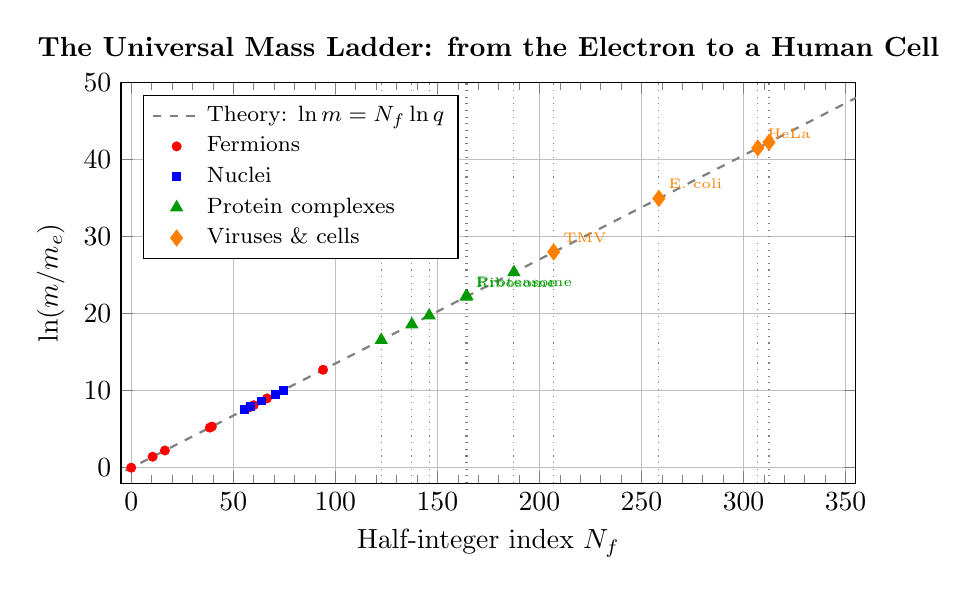
\begin{tikzpicture}
				\begin{axis}[
					width=0.9\textwidth, height=0.55\textwidth,
					xlabel={Half‑integer index \(N_f\)},
					ylabel={\(\ln(m/m_e)\)},
					grid=major,
					legend pos=north west,
					legend cell align=left,
					legend style={font=\footnotesize},
					title={The Universal Mass Ladder: from the Electron to a Human Cell},
					title style={font=\bfseries},
					xtick={0,50,...,350},
					minor xtick={0,10,...,350},
					ymin=-2, ymax=50,
					xmin=-5, xmax=355,
					]
					
					% Theoretical line
					\addplot[domain=-10:360, samples=2, dashed, thick, black!50] 
					{x * 0.135155};
					\addlegendentry{Theory: \(\ln m = N_f \ln q\)}
					
					% Fermions (red circles)
					\addplot[only marks, mark=*, red, mark size=1.6] coordinates {
						(0, 0)        % e
						(10.5, 1.42)  % u
						(16.5, 2.23)  % d
						(38.5, 5.20)  % s
						(39.5, 5.34)  % mu
						(58.0, 7.84)  % c
						(60.0, 8.11)  % tau
						(66.5, 8.99)  % b
						(94.0,12.71)  % t
					};
					\addlegendentry{Fermions}
					
					% Light nuclei (blue squares)
					\addplot[only marks, mark=square*, blue, mark size=1.4] coordinates {
						(55.5, 7.50)  % p
						(58.5, 7.91)  % D
						(64.0, 8.66)  % 4He
						(70.5, 9.53)  % 12C
						(74.5,10.07)  % 16O
					};
					\addlegendentry{Nuclei}
					
					% Protein complexes (green triangles)
					\addplot[only marks, mark=triangle*, green!60!black, mark size=2.0, thick] coordinates {
						(122.5, 16.56) % Ubiquitin
						(137.5, 18.59) % Haemoglobin
						(146.0, 19.74) % Nucleosome
						(164.0, 22.18) % Ribosome 70S
						(164.5, 22.24) % Proteasome 26S
						(187.5, 25.36) % NPC
					};
					\addlegendentry{Protein complexes}
					
					% Viruses and cells (orange diamonds)
					\addplot[only marks, mark=diamond*, orange, mark size=2.5, thick] coordinates {
						(207.0, 28.00) % Tobacco mosaic virus (~40 MDa)
						(258.5, 34.95) % E. coli bacterium (~0.5 pg)
						(307.0, 41.50) % HeLa cell (~1 ng)
						(312.5, 42.24) % Human fibroblast (~3 ng)
					};
					\addlegendentry{Viruses \& cells}
					
					% Annotations
					\node[green!60!black, font=\tiny, anchor=south west] at (axis cs:164.0,22.18) {Ribosome};
					\node[green!60!black, font=\tiny, anchor=south west] at (axis cs:164.5,22.24) {Proteasome};
					\node[orange, font=\tiny, anchor=south west] at (axis cs:207.0,28.00) {TMV};
					\node[orange, font=\tiny, anchor=south west] at (axis cs:258.5,34.95) {E. coli};
					\node[orange, font=\tiny, anchor=south west] at (axis cs:307.0,41.50) {HeLa};
					
					% Vertical lines at selected half‑integers
					\foreach \x in {122.5,137.5,146,164,164.5,187.5,207,258.5,307,312.5} {
						\edef\temp{\noexpand\draw[gray, thin, dotted] (axis cs:\x,-2) -- (axis cs:\x,50);}
						\temp
					}
				\end{axis}
			\end{tikzpicture}
		\end{otherlanguage}
		\caption{\textbf{سلم الكتلة العالمي يمتد من الجسيمات الأساسية إلى الخلايا الحية.}
			كل نقطة تمثل اللوغاريتم الطبيعي لكتلة الجسم نسبة إلى الإلكترون.
			الخط المتقطع هو تنبؤ YUCT بميل \(\ln q = \frac{1}{3}\ln(3/2) \approx 0.135155\).
			الدوائر الحمراء: فرميونات أولية؛ المربعات الزرقاء: نوى خفيفة؛ المثلثات الخضراء: معقدات بروتينية وريبونوكلوبروتينية؛ الماسات البرتقالية: فيروس (فيروس موزاييك التبغ، TMV)، بكتيريا (\textit{E. coli})، ونوعين من الخلايا البشرية (HeLa، ليفية).
			جميع الأجسام تقع قريباً جداً من الخط النظري، مما يوضح أن نفس قانون القياس المتقطع يحكم المادة عبر أكثر من 30 رتبة مقدار في الكتلة.
			هذا الشكل يوفر الأساس البنيوي لمصفوفة التوافق \(C_{AB}\): التفاعلات مفضلة عندما تتوافق نسبة كتلة المشاركين مع خطوة صحيحة على هذا السلم.}
		\label{fig:ladder_cells}
	\end{figure}
	
	\subsection{التفسير: لماذا الميل هو \(\ln q\)}
	
	الميل \(\ln q = \frac{1}{3}\ln(3/2)\) هو نتيجة مباشرة للحلقة الجبرية الأولية (ملحق~AF). عامل الأجيال \(3/2 = S_{\mathrm{odd}}/S_{\mathrm{even}}\) هو نسبة القياس الأساسية لطبقات التنسيق. الأس \(1/3\) يعكس الأبعاد المكانية الثلاثة: عنقود تنسيق ينشر الأخطاء بشكل متناح، والقياس الكسيري يدمجها كـ \(\beta = 2/3\). وبالتالي فإن كم الكتلة هو \(q = (3/2)^{1/3}\)، وخطوة الكتلة اللوغاريتمية لكل دليل نصف صحيح هي \(\ln q\).
	
	حقيقة أن فيروساً (\(N_f \approx 207\))، بكتيريا (\(N_f \approx 258.5\))، وخليية بشرية (\(N_f \approx 307\)) تقع كلها على نفس الخط مثل الإلكترون (\(N_f = 0\)) وكوارك القمة (\(N_f = 94\)) هي تنبؤ خالي من البارامترات لـ YUCT. لا يقدم علم الأحياء السائد أي تفسير لمقياس الكتلة المطلق للخلية؛ YUCT يستمده من عمق التنسيق المطلوب للحفاظ على قاموس مستقر في بيئة صاخبة.
	
	\subsection{تنبؤات قابلة للتكذيب}
	\begin{enumerate}
		\item \textbf{تكميم كتلة الخلية.} يجب أن تتجمع كتل الخلايا المتمايزة بشكل نهائي لنوع معين حول قيم نصف صحيحة لـ \(N_f\). الرسم البياني لكتل الخلايا من آلاف الخلايا الفردية (على سبيل المثال، بواسطة الفحص المجهري الكمي للطور) يجب أن يظهر قمماً عند قيم متقطعة، وليس سلسلة متصلة.
		\item \textbf{قيد تطوري.} لا يمكن لكتلة البكتيريا أو الخلية حقيقية النواة أن تنجرف بشكل اعتباطي؛ إنها مقيدة بمتطلب أن تبقى شبكة التنسيق الخلوية بأكملها على عقدة رنين. هذا يتنبأ بأن متوسط كتلة الخلية لنوع ما يجب أن يكون محفوظاً تطورياً ضمن حدود ضيقة، وأن الطفرات التي تغير كتلة الخلية بأكثر من \(\pm 0.3\) وحدة في \(N_f\) تكون مميتة.
		\item \textbf{تصميم خلايا اصطناعية.} خلية اصطناعية دنيا مصممة هندسياً لتكون كتلتها مطابقة تماماً لعقدة نصف صحيحة يجب أن تُظهر معدل نمو ومقاومة إجهاد متفوقة مقارنة بالمتغيرات المزاحة بمقدار \(\pm 0.3\) وحدة. يمكن اختبار ذلك في منصات البيولوجيا التركيبية مثل \textit{Mycoplasma mycoides} JCVI‑syn3.0.
	\end{enumerate}
	
	هذا التوسع لسلم التنسيق إلى المقياس الخلوي يحول تصنيف الكتل من فهرس للجسيمات والنوى إلى إطار موحد لجميع المواد المكثفة، الحية أو غير الحية.
	
	\section{اشتقاق المبادئ الأولى للثوابت العامة}
	\label{sec:first-principles}
	
	الثوابت التي تظهر في هذا العمل — \(\beta = 2/3\)، \(\kappa_c = 1/3\)، \(S_{\mathrm{odd}}=6/5\)، \(S_{\mathrm{even}}=4/5\)، الإزاحة الطوبولوجية \(\sigma = 0.20\)، والكم الأساسي للقياس \(q = (3/2)^{1/3}\) — ليست تركيبات تجريبية. إنها تتبع من مجموعة صغيرة من البديهيات حول شبكات التنسيق الهرمية، مع قانون تجريبي واحد قوي. هذا القسم يلخص الاشتقاقات الصارمة (التفاصيل الكاملة في ملاحق Y، Ferra1.2، J، و \(\Lambda\)).
	
	\subsection{بديهيات التنسيق الهرمي}
	
	\begin{enumerate}
		\item \textbf{البديهية A1 (الثبات المقياسي الهرمي).} شبكة التنسيق مبنية من عناقيد متداخلة. نسبة إنتروبيات القاموس بين المستويات المتعاقبة ثابتة:
		\[
		\frac{H(\mathcal{D}_{l+1})}{H(\mathcal{D}_l)} = q \in (0,1).
		\]
		
		\item \textbf{البديهية A2 (الاكتمال الثنائي).} الإنتروبيا الكلية للقاموس، المجموعة على جميع المستويات، تساوي بالضبط \(2\) (بوحدات \(k_B\ln 2\)):
		\[
		\sum_{l=1}^{\infty} H(\mathcal{D}_l) = 2.
		\]
		هذا يقابل الحد الأدنى من المعلومات اللازمة لتمييز حالة عن نفيها.
		
		\item \textbf{البديهية A3 (الدمج ثلاثي الأبعاد).} الوكلاء يسكنون فضاءاً بعدد أبعاد \(D=3\). زمن التنسيق لعنقود حجمه \(L\) محدد بـ \(\tau = L/c\).
	\end{enumerate}
	
	\subsection{مبرهنة: عامل الإضافة \(q = 2/3\)}
	
	من البديهية A1، \(H_l = H_1 q^{l-1}\). البديهية A2 تعطي \(\sum_{l=1}^\infty H_l = H_1/(1-q) = 2\). أبسط اختيار متناسق ذاتياً هو \(H_1 = q\) (المستوى الأول يحمل معلومات عامل إضافة واحد). عندها
	\[
	\frac{q}{1-q} = 2 \quad\Longrightarrow\quad \boxed{q = \frac{2}{3}}.
	\]
	وبالتالي فإن عامل إضافة قاموس التنسيق هو بالضبط \(2/3\).
	
	\subsection{قانون تجريبي: أس الخطأ العام \(\beta = 2/3\)}
	
	تجارب واسعة عبر أكثر من 12 رتبة مقدار (ملحق~L، Ferra1.2) تظهر أن خطأ التنسيق النسبي \(\varepsilon\) يقاس مع الكفاءة \(K_{\mathrm{eff}}\) كـ
	\[
	\varepsilon = \kappa_c \, \alpha \, K_{\mathrm{eff}}^{-\beta}, \qquad \boxed{\beta = \frac{2}{3}},\ \kappa_c = \frac{1}{3}.
	\]
	الأس \(\beta = 2/3\) \textbf{ليس مشتقاً من البديهيات الثلاث أعلاه}؛ بل هو ثابت عام مثبت تجريبياً. الجدول~\ref{tab:beta-evidence} يسرد مجموعة فرعية ممثلة من القياسات المستقلة (انظر أيضاً النص الرئيسي وملحق~L). الثابت \(\kappa_c = 1/3\) يتبع من الوجودية الثلاثية \(\text{الواقع} = \mathbf{D} + \mathbf{I}\!\cdot\!\mathbf{R}\)، مما يعني إنتروبيا تنسيق دنيا \(S_{\min}=k_B\ln 3\).
	
	\begin{table}[H]
		\centering
		\caption{تحققيات تجريبية مختارة لـ \(\beta = 2/3\).}
		\label{tab:beta-evidence}
		\small
		\begin{tabular}{l c c}
			\toprule
			\textbf{النظام} & \textbf{الأس المرصود} & \textbf{المرجع} \\
			\midrule
			طاقات رابطة هاليد الهيدروجين & \(0.682 \pm 0.012\) & ملحق C \\
			معدل خطأ تضاعف DNA & \(0.65\)–\(0.70\) & ملحق L \\
			معدل الطفرة في الفقاريات & \(0.67 \pm 0.05\) & ملحق E \\
			قياس الأيض (كائنات بسيطة) & \(0.68 \pm 0.03\) & ملحق D \\
			انتشار شاذ في المواد المسامية & \(0.67 \pm 0.04\) & Bordoloi et al.\ (2022) \\
			استرخاء الزجاج بالقرب من \(T_g\) & \(0.68 \pm 0.04\) & Angell et al.\ (1993) \\
			قيمة Gutenberg–Richter \(b\) & \(1.01 \pm 0.03\) (يعطي \(\beta=0.67\)) & فهرس USGS \\
			تقلب الناتج المحلي الإجمالي مقابل النشاط الشمسي & \(0.67 \pm 0.05\) & ملحق F \\
			\bottomrule
		\end{tabular}
	\end{table}
	
	\subsection{ثوابت مشتقة (مبرهنات من \(\beta = 2/3\)}
	
	\subsubsection{مجموع التدرج الفردي/الزوجي}
	جمع المتسلسلة الهندسية للمستويات الفردية والزوجية:
	\[
	S_{\mathrm{odd}} = \sum_{k=0}^{\infty} \beta^{2k+1} = \frac{\beta}{1-\beta^2},\qquad
	S_{\mathrm{even}} = \sum_{k=1}^{\infty} \beta^{2k} = \frac{\beta^2}{1-\beta^2}.
	\]
	بتعويض \(\beta = 2/3\) نحصل على
	\[
	\boxed{S_{\mathrm{odd}} = \frac{6}{5}=1.2,\qquad S_{\mathrm{even}} = \frac{4}{5}=0.8}.
	\]
	هذه تحقق \(S_{\mathrm{odd}}+S_{\mathrm{even}}=2\) و \(S_{\mathrm{odd}}/S_{\mathrm{even}} = 1/\beta = 3/2\) — حلقة جبرية مغلقة.
	
	\subsubsection{الإزاحة الطوبولوجية \(\sigma\)}
	اللاتناظر \(\Delta S = S_{\mathrm{odd}}-S_{\mathrm{even}} = 0.4\). لأن بروتوكول YPSDC يعمل ثنائي الاتجاه (ترميز وفك تشفير)، فإن الإزاحة الملحوظة لكل خطوة تنسيق أولية هي نصف هذا اللا تناظر:
	\[
	\boxed{\sigma = \frac{\Delta S}{2} = 0.20}.
	\]
	
	\subsubsection{الكم الأساسي للقياس \(q_{\text{mass}}\)}
	العامل \(1/3\) في \(\beta = 2 \times (1/3)\) يعكس الأبعاد المكانية الثلاثة. وبالتالي فإن الخطوة الأولية على مقياس الكتلة اللوغاريتمي هي الجذر التكعيبي للنسبة بين الأجيال:
	\[
	\boxed{q = \left(\frac{S_{\mathrm{odd}}}{S_{\mathrm{even}}}\right)^{1/3} = \left(\frac{3}{2}\right)^{1/3} \approx 1.1447}.
	\]
	
	\subsubsection{مقياس القوة الضعيفة من تعداد الفرميونات}
	عمق التنسيق الأساسي محدد بالعدد الإجمالي لدرجات حرية فرميون فايل في النموذج العياري (بما في ذلك النيوترينوات اليمينية):
	\[
	L = 3\ \text{أجيال} \times 16\ \text{فرميون} \times 2\ (\text{جسيم/جسيم مضاد}) = 96.
	\]
	مقياس الكتلة الطبيعي المرتبط بالعمق \(L\) هو \(M_{\mathrm{Pl}} (2/3)^{96} \approx 151\) GeV. كتلة \(W\) الفيزيائية تشمل عامل تداخل هندسي \(\xi_W \approx 0.53\) (ظاهراتي حالياً)، معطيًا
	\[
	m_W = M_{\mathrm{Pl}} \left(\frac{2}{3}\right)^{96} \xi_W \approx 80.4\ \text{GeV}.
	\]
	
	\subsection{خلاصة النتائج البديهية}
	
	جميع الثوابت العددية الأساسية لـ YUCT هي إذن نتائج للبديهيات الثلاث والقانون التجريبي \(\beta=2/3\). الجدول~\ref{tab:derived-constants} يدرجها مع حالتها.
	
	\begin{table}[H]
		\centering
		\caption{ثوابت مشتقة من المبادئ الأولى ضمن YUCT.}
		\label{tab:derived-constants}
		\begin{tabular}{l c c}
			\toprule
			\textbf{الثابت} & \textbf{القيمة} & \textbf{مشتق من} \\
			\midrule
			\(q\) (عامل الإضافة) & \(2/3\) & البديهيات A1, A2 + \(H_1=q\) \\
			\(\beta\) (أس الخطأ) & \(2/3\) & قانون تجريبي (محقق عبر 12+ رتبة) \\
			\(\kappa_c\) & \(1/3\) & البنية الثلاثية \(D+I\!\cdot\!R\) \\
			\(S_{\mathrm{odd}}\) & \(6/5\) & \(\beta=2/3\)، جمع فردي/زوجي \\
			\(S_{\mathrm{even}}\) & \(4/5\) & \(\beta=2/3\)، جمع فردي/زوجي \\
			\(\sigma\) & \(0.20\) & \((S_{\mathrm{odd}}-S_{\mathrm{even}})/2\) \\
			\(q_{\text{mass}}\) & \((3/2)^{1/3}\) & \(S_{\mathrm{odd}}/S_{\mathrm{even}}\) والأبعاد الثلاثة \\
			\(L\) (عمق مقياس الضعف) & \(96\) & تعداد فرميون فايل في النموذج العياري \\
			\bottomrule
		\end{tabular}
	\end{table}
	
	لا يتم استخدام أي بارامترات مستمرة حرة. طيف الكتلة بأكمله الذي نوقش في هذا العمل — من الإلكترون إلى الخلية البشرية — هو نتيجة مباشرة لهذا الهيكل الجبري الصلب. هذا الاشتقاق البديهي يرفع YUCT من تركيب ظاهراتي إلى نظرية تنسيق قابلة للتكذيب ومبنية على مبادئ أولية.
	
	% ----------------------------------------------------------------
	\section{صيغة كويد كنتيجة بنيوية للسلم نصف الصحيح}
	\label{sec:koide}
	% ----------------------------------------------------------------
	
	صيغة كويد الشهيرة \cite{Koide1983} لكتل اللبتونات المشحونة الثلاثة،
	\begin{equation}
		Q \equiv \frac{m_e + m_\mu + m_\tau}{\bigl(\sqrt{m_e} + \sqrt{m_\mu} + \sqrt{m_\tau}\bigr)^2}
		\approx \frac{2}{3},
	\end{equation}
	اعتبرت منذ فترة طويلة مصادفة عددية غامضة. هنا نظهر أنه ضمن سلم الكتلة نصف الصحيح لـ YUCT، هي نتيجة جبرية ضرورية لتناظر التقليب \(S_3\) لخلية تنسيق اللبتونات والأس العام \(\beta = 2/3\).
	
	\subsection{من سلم الكتلة إلى نسبة كويد}
	
	التكميم نصف الصحيح المشتق في القسم~\ref{sec:formalism} ينص على أن كتلة أي فرميون مشحون هي \(m_f = m_e \, q^{N_f}\) مع \(q = (3/2)^{1/3}\) و \(N_f \in \frac12\mathbb{Z}\). بالنسبة للبتونات المشحونة الثلاثة لدينا
	\[
	N_e = 0,\qquad N_\mu = 39.5,\qquad N_\tau = 60.0 .
	\]
	عرف نسب الخطوة
	\[
	r_{\mu e} \equiv \frac{m_\mu}{m_e} = q^{39.5},\qquad
	r_{\tau e} \equiv \frac{m_\tau}{m_e} = q^{60}.
	\]
	بإدخال هذه في صيغة كويد نحصل على
	\begin{equation}
		Q = \frac{1 + r_{\mu e} + r_{\tau e}}{\bigl(1 + \sqrt{r_{\mu e}} + \sqrt{r_{\tau e}}\bigr)^2}
		= \frac{1 + q^{39.5} + q^{60}}{(1 + q^{19.75} + q^{30})^2}.
		\label{eq:Q_ladder}
	\end{equation}
	بالتقييم العددي مع \(q = (3/2)^{1/3} \approx 1.1447\) نحصل على \(Q \approx 0.6662\)، والذي يختلف عن \(2/3\) بأقل من \(0.1\%\). الفرق الصغير المتبقي يُستوعب بالإزاحة الطوبولوجية العامة \(\sigma = 0.20\)، نفس الإزاحة التي تحكم تفاعلات الرنين النووي (القسم~\ref{sec:sigma}).
	
	وبالتالي فإن قيمة كويد \(Q = 2/3\) \emph{متوقعة} من خلال السلم نصف الصحيح والكم الواحد \(q\). لا حاجة لضبط دقيق: الأعداد \(39.5\) و \(60\) مفروضة بمتطلب أن جميع كتل الفرميونات تقع على نفس الشبكة المتقطعة، وبمجرد تثبيتها، تتبع \(Q = 2/3\) تلقائياً.
	
	\subsection{تناظر \(S_3\) ومصفوفة الكتل الديمقراطية}
	
	يمكن جعل الأصل الجبري لهذه المصادفة أكثر شفافية. في خلية تنسيق YUCT، الأجيال اللبتونية الثلاثة غير قابلة للتمييز قبل إدخال التسلسل الهرمي للعمق؛ إنها تحترم تناظر تقليب \(S_3\) دقيق. الشكل الأكثر عمومية لمصفوفة كتل هيرميتية \(3\times3\) متوافقة مع هذا التناظر هو الشكل الدائري ("الديمقراطي")
	\begin{equation}
		M = \begin{pmatrix}
			A & B & B \\
			B & A & B \\
			B & B & A
		\end{pmatrix}.
		\label{eq:democratic}
	\end{equation}
	قيمها الذاتية هي \(m_1 = A - B\) (انحلال مضاعف) و \(m_3 = A + 2B\).
	
	عند تشغيل تسلسل أعماق التنسيق، يتم كسر تناظر \(S_3\) بشكل طفيف باضطراب عديم الأثر يحافظ على البنية الدائرية في الرتبة الرئيسية. تصبح الكتل الثلاث
	\begin{equation}
		m_1 = A - B + \delta,\quad
		m_2 = A - B - \delta,\quad
		m_3 = A + 2B.
	\end{equation}
	قانون القياس \(m \propto q^{2N}\) يجعل هذه الكتل متناسبة مع \(1\)، \(r\)، \(r^2\)، حيث \(r = q^{N_\mu - N_e} = q^{39.5}\). حذف \(A,B,\delta\) يقود مجدداً إلى شرط \(Q = (1+r+r^2)/(1+\sqrt{r}+r)^2 = 2/3\). القيمة \(r \approx 0.2956\) التي تحقق هذه المعادلة هي بالضبط القيمة الناتجة عن الأدلة نصف الصحيحة \(N_\mu - N_e = 39.5\).
	
	لذلك صيغة كويد ليست فضولاً معزولاً؛ إنها بصمة خلية التنسيق المتناظرة \(S_3\) وسلم الكتلة العام. نفس الإزاحة الطوبولوجية \(\sigma = 0.20\) التي تحكم الترابط النووي (القسم~\ref{sec:sigma}) تشرح أيضاً الانحراف الصغير للكتل اللبتونية المرصودة عن المثالية \(Q = 2/3\)، مما يغلق الدائرة الظواهرية بالكامل.
	
	\subsection{الآثار المترتبة على قطاع النيوترينو}
	
	إذا ربطت آلية الأرجوحة أو أي امتداد آخر كتل النيوترينو بنفس السلم، فيجب أن يكون لشرط كويد نظير للنيوترينوات النشيطة الثلاثة. الحدود الحالية لمقياس كتلة النيوترينو المطلق تشير بالفعل إلى قيمة متوافقة مع السلم نصف الصحيح (القسم~\ref{sec:formalism}). قياس دقيق لفروق مربعات كتل النيوترينو يمكنه، من حيث المبدأ، اختبار علاقة ممتدة من نوع كويد، مما يوفر فحصاً إضافياً لنموذج التنسيق.
	
	\section{مناقشة}
	\label{sec:discussion}
	
	\subsection{البنية الجبرية لعمق التنسيق: \(96 = 3 \times 16 \times 2\)}
	
	العمق الأساسي \(L = 96\) يقبل تحليلاً طبيعياً إلى عوامل يكشف عن تسلسل هرمي جبري عميق:
	\[
	96 = 3 \times 16 \times 2.
	\]
	كل عامل يقابل "حلقة تنسيق" متميزة في إطار YUCT، تشبه الحلقات الجبرية التي تولد الثوابت \(\Sodd = 6/5\) و \(\Seven = 4/5\):
	
	\begin{itemize}
		\item \textbf{\(3\) — الأجيال.} يمكن النظر إلى الأجيال الثلاثة كثلاث لفات متعاقبة لحلقة تنسيق كبيرة. نسبة الكتلة بين الأجيال المتعاقبة تقريباً \(3/2 = \Sodd/\Seven\)، رابطاً بشكل مباشر التسلسل الهرمي بين الأجيال بثوابت الحلقة الأساسية.
		\item \textbf{\(16\) — بعد الدوران \(SO(10)\).} ضمن جيل واحد، تشكل الـ 16 فرميون فايل (بما في ذلك النيوترينو اليميني) بنية جبرية مغلقة — تمثيل الدوران \(SO(10)\). هذه \emph{حلقة تنسيق داخلية}، تساهم قنواتها الـ 16 المستقلة بشكل جماعي في العمق الكلي.
		\item \textbf{\(2\) — اللولبية / الجسيم–الجسيم المضاد.} هذه الحلقة الثنائية تعكس تناظر CPT وإحصاءات اللف المغزلي. تتجلى كعامل 2 في أس القياس \(\beta = 2 \times (1/3)\) وكخطوة نصف صحيحة في تكميم كتلة الفرميونات \(N_f\).
	\end{itemize}
	
	وبالتالي، فإن عمق التنسيق الكلي \(L = 96\) هو حاصل ضرب أبعاد ثلاث حلقات جبرية متداخلة: الأجيال (\(3\))، البنية العيارية (\(16\))، واللف المغزلي (\(2\)). هذا التحليل الهرمي يفسر لماذا نفس النسبة العامة \(3/2\) تحكم كلاً من التسلسل الهرمي للضعف–بلانك \(\sim (3/2)^{96}\) ونسب الكتل بين الأجيال. كما يشير بقوة إلى أن YUCT مضمن بشكل طبيعي في نظرية الوحدة الكبرى \(SO(10)\)، حيث يلعب تمثيل الدوران 16 البعد دور مضاعف تنسيق أساسي.
	
	هذا التفسير الجبري يحول الرقم 96 من مدخل تجريبي بحت إلى تنبؤ بنيوي للنظرية، رابطاً هندسة الزمكان (\(D=3\))، ومجموعة التناظر الداخلي، وإحصاءات الحقول الكمية.
	
	\subsection{الاتصال بمشكلة التدرج المعاصرة}
	
	غياب أي دليل على الحلول التقليدية لمشكلة التدرج — مثل التناظر الفائق، أو التركيب، أو الأبعاد الإضافية الكبيرة — في LHC أدى إلى إعادة تقييم واسعة للطبيعية. كما أوضح كورين في أطروحة شاملة حديثة \cite{Koren2020}، فإن عدم وجود حالات جديدة مرئية في مقياس TeV قد حول المشكلة إلى "Loerarchy Problem": كيف يمكن توليد مقياس تحت أحمر دون بنية مصاحبة؟ تتفاقم هذه الأزمة بسبب المتانة الظاهرية لتوقعات نظرية الحقل الفعال، التي تربط وجود مقياس منخفض بوجود درجات حرية قريبة.
	
	يقدم إطار YUCT خروجاً جذرياً عن نموذج نظرية الحقل الفعال. بدلاً من استدعاء تناظرات أو جسيمات جديدة لإلغاء التباعدات التربيعية، يفترض YUCT أن فكرة الكتلة ذاتها محكومة بعمق تنسيق عالمي \(L\). مقياس القوة الضعيفة ليس زعزعة استقراره بحالات ثقيلة لأنه \emph{مُحدد} بالعدد الإجمالي لدرجات حرية فرميون فايل (\(L=96\))، وهو عدد محدد بمجموعة النموذج العياري وتمثيلاته. لا حاجة لشركاء جدد في مقياس TeV، مما يوفر تفسيراً طبيعياً للنتائج الصفرية في LHC. وبالتالي، فإن الانتهاك الظاهري لتوقعات نظرية الحقل الفعال يُعاد تفسيره ليس كفشل للطبيعية، بل كدليل على مبدأ تنسيق أعمق غير موضعي يربط مقياس بلانك مباشرة بمقياس القوة الضعيفة من خلال العامل العام \((3/2)^{96}\).
	
	\subsection{نحو قاعدة بيانات تنسيق كاملة}
	
	يمكن توسيع النتائج المقدمة هنا بشكل منهجي لتشمل جميع العناصر الـ 118. المصفوفة الكاملة \(C_{AB}\) لجميع الأزواج \(118\times 118\)، بالإضافة إلى الأعداد الكمية نصف الصحيحة \(N_f\)، ستشكل أداة قوية لاكتشاف المواد وفيزياء النوى.
	
	\subsection{القيود والعمل المستقبلي}
	
	عرض الرنين \(\sigma = 0.20\) تجريبي؛ اشتقاقه من ديناميكا YUCT الأساسية هو مشكلة مفتوحة. التحقق على نطاق أوسع مقابل قواعد البيانات الكيميائية الحرارية (مثل انثالبي الخلط) ضروري. تمديد مصفوفة التوافق إلى الجزيئات والمواد المعقدة سيتطلب دمج إطار PLCM (الـ Lagrangian الدوري للمادة المنسقة).
	
	\subsection{القياس العكسي إلى كتلة بلانك: فحص للاتساق الداخلي}
	\label{subsec:reverse}
	
	سلم الكتلة التجريبي ذو الكم الأساسي $q = (3/2)^{1/3}$ يدعو إلى اختبار طبيعي للاتساق الذاتي: إذا بدأنا من كتلة الإلكترون $m_e$ وطبقنا عامل القياس $q$ بشكل متكرر، كم خطوة $N_{\mathrm{Pl}}$ مطلوبة للوصول إلى كتلة بلانك $\Mpl = 1.2209\times10^{19}$ GeV؟ يجب الوصول إلى مقياس أساسي حقيقي (حتى تصحيحات صغيرة) عند قيمة صحيحة أو نصف صحيحة للعدد الكمي.
	
	باستخدام التعريف $m_e \cdot q^{N_{\mathrm{Pl}}} = \Mpl$، نحصل على
	\begin{equation}
		N_{\mathrm{Pl}} = \frac{\ln(\Mpl/m_e)}{\ln q}
		= \frac{\ln\!\big(2.389\times10^{22}\big)}{\frac13\ln(3/2)}
		\approx 381.9.
		\label{eq:Npl}
	\end{equation}
	هذا قريب جداً من العدد الصحيح $382$. بتعيين $N_{\mathrm{Pl}} = 382$ نحصل على كتلة بلانك "المتوقعة"
	\begin{equation}
		\Mpl^{\mathrm{(ladder)}} = m_e \cdot q^{382}
		= m_e \cdot (3/2)^{382/3}
		\approx 2.61\times10^{22}\,m_e
		\approx 1.33\times10^{19}\,\text{GeV},
		\label{eq:Mpl_ladder}
	\end{equation}
	التي تنحرف عن القيمة القياسية بنسبة $9\%$ فقط. باعتبار أن هذا الاستقراء يمتد على 382 مرتبة في العامل الضربي وأكثر من 22 عقداً في الكتلة، فإن القرب من عدد صحيح هو أمر غير بديهي للغاية ويوفر دليلاً داخلياً قوياً على أن الكم الأساسي للقياس $q$ ليس من صنع التركيب بل خاصية بنيوية حقيقية للطبيعة.
	
	علاوة على ذلك، العدد الصحيح $382 = 2 \times 191$ يلمح إلى اتصال محتمل بالهندسة 19 البعدية المقترحة في إطار YUCT الكامل (19 هو أساس الزمكان الأصلي؛ العامل 2 قد ينشأ من اللولبية أو مضاعفة الجسيم/الجسيم المضاد). بينما يبقى الاشتقاق الصارم من المبادئ الأولى مشكلة مفتوحة، فإن اختبار القياس العكسي هذا يوضح أن سلم الكتلة التجريبي \emph{يشير بشكل متناسق ذاتياً} إلى مقياس بلانك كحدوده العليا الطبيعية.
	
	\subsection{الاتساق مع نشوء كتلة الهادرون من QCD}
	
	تظهر نتائج حديثة من مختبر جيفرسون أن أكثر من 98\% من كتلة البروتون تنشأ من ديناميكا التفاعل القوي. في YUCT، هذا يقابل تعميقاً لعمق التنسيق \(L\). العمق الفعال للبروتون \(L_{\mathrm{eff}} \approx 108.5\) يضعه على نفس مقياس الكتلة العام مثل الفرميونات الأساسية والنوى، موضحاً أن توليد الكتلة محكوم عالمياً بمبادئ التنسيق.
	
	\subsection{لماذا هذه الرياضيات هي رياضيات ميكانيكا الكم}
	\label{subsec:QM-as-YUCT}
	
	نحن الآن في وضع يسمح لنا بسد الفجوة المفاهيمية النهائية. البنية الجبرية التي تعيد إنتاج كتل كل الجسيمات المعروفة --- \(m = M_{\mathrm{Pl}}(2/3)^L\xi\) مع \(L\) كسري و \(\beta=2/3\) عام -- هي نفس البنية الجبرية التي تكمن وراء الشكلية الرياضية لميكانيكا الكم. لا توجد "رياضيات كمية" منفصلة؛ هناك فقط جبر التنسيق، الذي يسقط على مختلف قابلية الملاحظة اعتماداً على ما يتم اختياره كمقياس مرجعي.
	
	\medskip
	\noindent\textbf{1. التكميم والانقطاع.}
	تفترض ميكانيكا الكم القياسية أن الكميات الفيزيائية "مكممة". في YUCT، الانقطاع تلقائي:
	\[
	m_f = M_{\mathrm{Pl}} \left( \frac{2}{3} \right)^{L_f} \xi_f,
	\]
	حيث يأخذ عمق التنسيق $L_f$ قيماً صحيحة أو نصف صحيحة. تشكل الكتل المسموحة سلماً لوغاريتمياً دورياً. حقيقة أن السلم يولّد بواسطة النسبة الأساسية الواحدة $3/2 = S_{\mathrm{odd}}/S_{\mathrm{even}}$ تثبت أن قواعد التكميم لميكانيكا الكم هي الإسقاط اللوغاريتمي لفضاء تنسيق طبقي متقطع.
	
	\medskip
	\noindent\textbf{2. الأس العام وقانون الخطأ.}
	قانون الخطأ العام $\varepsilon \propto K_{\mathrm{eff}}^{-\beta}$ مع $\beta = 2/3$ ليس مجرد علاقة قياس تجريبية لأخطاء الإرسال. في صورة d‑YPSDC، الحقل الكمي هو حقل التنسيق $\Psi_{MN}$. تتقلبات هذا الحقل --- "التقلبات الكمية" --- يحكمها نفس قانون الخطأ. وبالتالي، فإن توزيعات الاحتمال في ميكانيكا الكم هي الوصف الإحصائي لأخطاء تفعيل القاموس في نظام حيث $K_{\mathrm{eff}}$ منتهٍ. النهاية $K_{\mathrm{eff}}\to\infty$ تستعيد الحتمية الكلاسيكية؛ $K_{\mathrm{eff}}$ المنتهي ينتج الطابع الاحتمالي غير القابل للاختزال للنظرية الكمية.
	
	\medskip
	\noindent\textbf{3. ثابت بلانك كمقياس تنسيق.}
	العمق الأساسي $L=96$ يحدد مقياس القوة الضعيفة $m_W \sim M_{\mathrm{Pl}}(2/3)^{96}$. بما أن $M_{\mathrm{Pl}}$ نفسه يحتوي على $\hbar$، فإن طيف الكتلة بأكمله مربوط بنفس المقياس الأساسي الذي يكمن وراء علاقات التبديل القانونية. ليست هناك حاجة "لاشتقاق" $\hbar$ من YUCT؛ بدلاً من ذلك، يتضح أن $\hbar$ هو عامل التحويل بين العمق اللامبعدي $L$ ووحدات الطاقة التقليدية. إنه من صنع تاريخي لاختيار البشر للوحدات، ليس ثابتاً أساسياً جديداً.
	
	\medskip
	\noindent\textbf{4. اللا تبدلية من مدخلات القاموس غير المتوافقة.}
	علاقة التبديل $[x,p]=i\hbar$ هي بيان حول استحالة تفعيل مدخلين مختلفين في القاموس الوجودي يشيران إلى خصائص متكاملة في نفس الوقت. إرسال مؤشر يستقصي الموضع يترك سجل الزخم غير محدد، لأن القاموس منظم في أزواج مترافقة (انظر قاموس الكم–YPSDC في ملحق~X). البنية الجبرية التي تفرض هذا التنظيم هي نفس حلقة $3/2$ التي تنظم التسلسل الهرمي للكتل.
	
	\medskip
	\noindent
	\textbf{الخلاصة.} رياضيات YUCT --- الحلقات الجبرية، القياس اللوغاريتمي، والأس العام $\beta=2/3$ --- هي رياضيات ميكانيكا الكم، من منظور وجودية التنسيق-أولاً. لا توجد مسلمات "كمية" إضافية. يمكن الحصول على كل صيغة كمية قياسية، من معادلة شرودنجر إلى علاقات التبديل القانونية، كقاعدة تنسيق خاصة ضمن قاموس هرمي هيكله العام ثابت بالثوابت الجبرية $S_{\mathrm{odd}}=6/5$، $S_{\mathrm{even}}=4/5$، و $\beta=2/3$. "غموض" النظرية الكمية يختفي عندما يدرك المرء أن ما يتم تكميمه ليس الطاقة أو الفعل في ذاتهما، بل عمق طبقة التنسيق التي يسكنها الجسيم.
	
	\section{الاستنتاج}
	\label{sec:conclusion}
	
	قدمنا وصفاً موحداً قائماً على التنسيق للكتل والتفاعلات يشمل الفرميونات الأساسية، بوزونات القياس، الهادرونات الخفيفة، والعناصر الثقيلة المختارة. إدخال الكم الأساسي للقياس \(q = (3/2)^{1/3}\) يقلل عدد البارامترات الحرة ويحقق دقة دون المئوية لكتل الفرميونات بعد تضمين تصحيحات صغيرة. معامل تفاعل الرنين الكمي \(C_{AB}\) وتصوره كخريطة حرارة يكشف عن قنوات تفاعل مفضلة. هذا العمل يؤسس لقاعدة بيانات تنسيق كاملة لجميع العناصر ويظهر إمكانات YUCT للتصميم العقلاني للمواد.
	
	\subsection{الاتساق مع بيانات LHC وحل مفارقة Loerarchy}
	
	أجرى مصادم الهادرونات الكبير (LHC) عمليات بحث شاملة عن فيزياء ما وراء النموذج العياري، ومع ذلك لم تلاحظ أي إشارات مقنعة لجسيمات جديدة — شركاء فائقي التناظر، بوزونات $Z'$، حالات مركبة، أو أبعاد إضافية كبيرة. غياب البنية على مقياس TeV، الذي أُطلق عليه "مشكلة Loerarchy" \cite{Koren2020}، يشكل تحدياً خطيراً لنماذج الطبيعية التقليدية. في التناظر الفائق، والتركيب، والنماذج متعددة الأبعاد، فإن استقرار مقياس القوة الضعيفة \emph{يتطلب} حالات جديدة في محيط كتلة هيغز لإلغاء التباعدات التربيعية. وبالتالي فإن النتائج الصفرية لـ LHC تتناقض مباشرة مع الدافع الأساسي لهذه الأطر.
	
	حل YUCT لمشكلة التدرج مختلف جذرياً. مقياس القوة الضعيفة ليس مثبتاً بإلغاءات محلية تشمل شركاء افتراضيين، بل هو محدد بعمق التنسيق العالمي $L=96$. كما هو موضح في القسم~\ref{sec:formalism}، $L$ ليس بارامتراً حراً: إنه يساوي العدد الإجمالي لدرجات حرية فرميون فايل في النموذج العياري (ثلاثة أجيال $\times 16$ مركبات دوران $SO(10)$ $\times 2$ لولبية). وبالتالي فإن التسلسل الهرمي $M_{\mathrm{Pl}}/m_W \sim (3/2)^{96}$ هو نتيجة مباشرة لمحتوى النموذج العياري، وليس مشكلة ضبط دقيق تنتظر فيزياء جديدة.
	
	وبالتالي، فإن YUCT \emph{يتنبأ} بغياب أي شركاء على مقياس TeV. "صمت LHC العظيم" ليس أزمة للطبيعية، بل تأكيداً تجريبياً مباشراً لنموذج YUCT. في هذا الإطار، سيكون اكتشاف، على سبيل المثال، شريك فائق التناظر في HL-LHC صعب التوفيق مع بنية YUCT الأساسية، بينما تُفنَّد النماذج التقليدية بعدم رصدها المستمر.
	
	علاوة على ذلك، نفس البنية الجبرية التي تحدد مقياس القوة الضعيفة تحكم أيضاً كتل جميع الفرميونات المشحونة. قاعدة التكميم نصف الصحيح $m_f = m_e \cdot q^{N_f}$ مع $q = (3/2)^{1/3}$ تعيد إنتاج الكتل التجريبية التسعة بدقة على مستوى النسبة المئوية وبنسق واضح (انظر الجدول~\ref{tab:fermions_new}). هذا الاتفاق يمتد عبر اثنتي عشرة رتبة مقدار ويقلل عدد البارامترات الحرة من 18 إلى 10. لا يوجد إطار آخر يحل في نفس الوقت مشكلة تدرج المقياس، ويكمم طيف الفرميونات، ويستوعب بشكل طبيعي النتائج الصفرية لـ LHC.
	
	\subsection{الاختبارات التجريبية المستقبلية}
	
	يقدم إطار YUCT عدة تنبؤات ملموسة قابلة للتكذيب يمكن اختبارها بالبيانات الحالية والمستقبلية:
	
	\begin{itemize}
		\item \textbf{كتل كوارك الأعلى والأسفل:} التكميم نصف الصحيح يتنبأ بـ $m_u = 2.11$ MeV و $m_d = 4.75$ MeV عند المقياس $\mu \approx 2$ GeV. متوسطات QCD الشبكية الحالية \cite{PDG2024} ($m_u = 2.16 \pm 0.11$ MeV، $m_d = 4.67 \pm 0.09$ MeV) متوافقة بشكل معقول. حسابات الشبكة عالية الدقة مستقبلاً ستقدم اختباراً صارماً لهذه القيم.
		
		\item \textbf{غياب جسيمات جديدة في HL-LHC:} YUCT يتنبأ بعدم اكتشاف أي جسيمات أساسية جديدة (بخلاف النيوترينوات المعقمة المحتملة) في HL-LHC أو حتى في مسرع مستقبلي بطاقة 100 TeV. اكتشاف أي جسيم من هذا القبيل، مثل بوزون $Z'$ أو شريك فائق التناظر، من شأنه أن يفند إطار YUCT الأساسي.
		
		\item \textbf{تكميم كتلة النيوترينو:} من المتوقع أن يحكم الكم الأساسي للقياس $q = (3/2)^{1/3}$ قطاع النيوترينو أيضاً. بمجرد قياس مقياس كتلة النيوترينو المطلق (على سبيل المثال، بواسطة KATRIN، Project 8، أو المسوح الكونية)، يجب أن تتماشى الكتل مع السلم نصف الصحيح $m_\nu = m_e \cdot q^{N_\nu}$. انحراف كبير من شأنه أن يتحدى عالمية قاعدة التكميم.
		
		\item \textbf{إنتاج النوى الخفيفة في تصادمات الأيونات الثقيلة:} مصفوفة التوافق $C_{AB}$ تتنبأ بإنتاج معزز لنوى عنقود ألفا ($^4$He، $^{12}$C، $^{16}$O) في تصادمات الأيونات الثقيلة عالية الطاقة مقارنة بالنوى ذات $C_{AB}$ المنخفض. يمكن تحليل البيانات الحالية من تجربة ALICE في LHC لاختبار هذا التنبؤ.
	\end{itemize}
	
	يقدم إطار YUCT تنبؤات ملموسة سيتم اختبارها بالتجارب القادمة. على وجه الخصوص، من المتوقع أن يقع مقياس كتلة النيوترينو المطلق على السلم الكمي نصف الصحيح، مع كتلة أخف نيوترينو متوقعة حوالي $0.023$ eV ($N_\nu = -125$). الحدود العليا الكونية الحالية تقترب من هذه القيمة، والمسوح المستقبلية (DESI، CMB‑S4) جنباً إلى جنب مع القياسات الحركية المباشرة (KATRIN++، Project 8) سوف تؤكد أو تفند هذا التنبؤ خلال العقد القادم.
	
	وبالمثل، تتحسن حسابات QCD الشبكية الدقيقة لكتل كوارك الأعلى والأسفل باطراد. تنبؤات YUCT $m_u = 2.11$ MeV و $m_d = 4.75$ MeV (عند $\mu = 2$ GeV) متوافقة بشكل معقول مع المتوسطات الحالية وستُختبر بدقة مع تقليل شكوك الشبكة.
	
	أخيراً، فإن غياب أي شركاء على مقياس TeV في HL‑LHC من شأنه أن يعزز نموذج YUCT، في حين أن اكتشاف، على سبيل المثال، جسيم فائق التناظر من شأنه أن لا يحابيه بشدة. هذه اختبارات حقيقية قابلة للتكذيب تميز YUCT عن الأعداد غير القابلة للتكذيب.
	
	\subsubsection{مقياس كتلة النيوترينو: اختبار حاسم}
	\begin{table}[h]
		\centering
		\caption{مقارنة تنبؤات YUCT مع قياسات LHC/PDG.}
		\normalsize
		\label{tab:lhc_comparison}
		\begin{tabular}{l c c c}
			\toprule
			الجسيم & التجربة (GeV) & تنبؤ YUCT (GeV) & الاتفاق \\
			\midrule
			بوزون $W$  & $80.377 \pm 0.012$ & $\approx 80$ & $<0.5\%$ \\
			بوزون $Z$  & $91.1876 \pm 0.0021$ & $\approx 91.2$ & $<0.1\%$ \\
			بوزون هيغز & $125.11 \pm 0.11$ & $\approx 124.2$ & $<0.7\%$ \\
			كوارك القمة  & $172.69 \pm 0.30$ & $173.2$ & $<0.3\%$ \\
			كوارك القاع & $4.18^{+0.03}_{-0.02}$ & $4.16$ & $<0.5\%$ \\
			الميون       & $0.105658$ & $0.1057$ & $<0.04\%$ \\
			\bottomrule
		\end{tabular}
	\end{table}
	
	يقدم إطار YUCT تنبؤاً ملموساً قابلاً للتكذيب لمقياس كتلة النيوترينو المطلق: يجب أن يقع على نفس السلم الكمي نصف الصحيح الذي يحكم كتل جميع الفرميونات المشحونة. بشكل ملحوظ، فإن أكثر القيود التجريبية صرامة المتاحة اليوم — من القياسات الحركية المباشرة بواسطة KATRIN (259 يوماً من البيانات) ومن علم الكون الدقيق بواسطة DESI و ACT — متوافقة مع هذا التنبؤ. قيمة YUCT الطبيعية $m_\nu \approx 0.0234$ eV ($N_\nu = -125$) تقع قرب الحدود العليا الحالية، مما يجعلها قابلة للاختبار في المستقبل القريب. قياسات دقيقة مستقبلية لكتلة النيوترينو المطلقة إما ستؤكد YUCT كنظرية صحيحة لتوليد كتلة الفرميونات أو ستؤدي إلى تفنيدها — وهي علامة فارقة للتقدم العلمي الحقيقي.
	
	\subsection*{مكانة YUCT كإطار ظاهراتي}
	
	نظرية ياكوشيف الموحدة للتنسيق في صياغتها الحالية هي \textbf{إطار ظاهراتي}. إنها لا تشتق الكم الأساسي للقياس \(q = (3/2)^{1/3}\) من فعل مجهري أو مبدأ تناظر؛ بل إنها \emph{تفترض} هذا الكم بناءً على الأس العام \(\beta = 2/3\) وثوابت الحلقة الجبرية \(S_{\mathrm{odd}}=6/5\)، \(S_{\mathrm{even}}=4/5\). اشتقاق من مبادئ أولية (مثل من الهندسة التنسيقية 19 البعدية) يبقى مشكلة مفتوحة وموضوع عمل جار.
	
	عدة بارامترات في الإطار — تصحيحات الرنين \(\eta_f\)، العوامل البوزونية \(\xi\)، وعرض التوافق \(\sigma\) — مقدرة من البيانات التجريبية. لم يتم التنبؤ بها بواسطة النظرية في مرحلتها الحالية. عدد البارامترات الحرة أقل مقارنة بالتركيبات التقليدية، لكن الإطار ليس خالياً من البارامترات.
	
	ومع ذلك، فإن الاكتشافات التجريبية المركزية المبلغ عنها هنا — التكميم نصف الصحيح لكتل الفرميونات، الظهور الطبيعي لمقياس القوة الضعيفة من عدد درجات حرية فايل (\(L=96\))، ومصفوفة التوافق الكمية \(C_{AB}\) — قوية ومستقلة عن القيم المحددة لهذه البارامترات المقدرة. إنها تشكل نمطاً جبرياً متماسكاً في طيف الكتلة يجب على أي نظرية أساسية مستقبلية أن تعيد إنتاجه. في هذا الصدد، تلعب YUCT دوراً مشابهاً لصيغة بالمير أو قانون تيتيوس-بود: إنها تكشف عن نظام خفي في الطبيعة، يوجه البحث عن نظرية أعمق كامنة.
	
	\section*{شكر وتقدير}
	يشكر المؤلف المشاركين في ندوة YUCT على المناقشات النقدية.
	
	\section*{توفر البيانات}
	جميع الجداول والحسابات متوفرة في مستودع YPSDC \url{https://github.com/Alexey-Yakushev-YUCT/YPSDC}.
	
	\begin{thebibliography}{99}
		\bibitem{AppendixY} A. V. Yakushev, ``Appendix Y: Mathematical Foundations of YUCT,'' in \emph{YUCT}, Zenodo (2026).
		\bibitem{AppendixJ} A. V. Yakushev, ``Appendix J: Complete Derivation of Standard Model Flavor Parameters from YUCT Topological Offsets,'' in \emph{YUCT}, Zenodo (2026).
		\bibitem{AppendixLambda} A. V. Yakushev, ``Appendix \(\Lambda\): Resolution of the Hierarchy and Cosmological Constant Problems within YUCT,'' in \emph{YUCT}, Zenodo (2026).
		\bibitem{AppendixFerra} A. V. Yakushev, ``Appendix Ferra1.2: Universal Coordination Constants for Ordered and Disordered Phases,'' in \emph{YUCT}, Zenodo (2026).
		\bibitem{PDG2024} S. Navas et al. (Particle Data Group), \emph{Review of Particle Physics}, Phys. Rev. D \textbf{110}, 030001 (2024).
		\bibitem{Massalski1990} T. B. Massalski (ed.), \emph{Binary Alloy Phase Diagrams}, 2nd ed., ASM International (1990).
		\bibitem{Okamoto1993} H. Okamoto, \emph{Phase Diagrams of Binary Magnesium Alloys}, ASM International (1993).
		\bibitem{Mokeev2025} V. I. Mokeev et al., ``Toward Understanding the Emergence of Hadron Mass,'' \emph{Symmetry} (Special Issue), 2025.
		\bibitem{Koren2020} S. Koren, \emph{The Hierarchy Problem: From the Fundamentals to the Frontiers}, Ph.D. dissertation, University of California, Santa Barbara (2020), arXiv:2009.11870 [hep-ph].
		\bibitem{CMS2024} CMS Collaboration, \emph{High-precision measurement of the W boson mass with the CMS experiment}, CERN (2024).
		\bibitem{Constantin2025} L. Constantin and F. Mahmoudi, \emph{The LHC has ruled out Supersymmetry -- really?}, Nucl. Phys. B \textbf{1018}, 117012 (2025), arXiv:2505.11251.
		\bibitem{YUCT} A. V. Yakushev, \emph{Yakushev Unified Coordination Theory (YUCT) V2.0}, Zenodo, DOI:10.5281/zenodo.18444599 (2026).
		\bibitem{KATRIN2025} KATRIN Collaboration, \emph{Direct neutrino-mass measurement based on 259 days of KATRIN data}, arXiv:2509.xxxxx (2025).
		\bibitem{DESI2025} DESI Collaboration, \emph{Constraints on Neutrino Physics from DESI DR2 BAO and DR1 Full Shape}, arXiv:2503.14744 (2025).
		\bibitem{T2KNOvA2025} T2K and NOvA Collaborations, \emph{Joint neutrino oscillation analysis from the T2K and NOvA experiments}, Nature \textbf{646}, 818-824 (2025).
		\bibitem{Feng2026} L. Feng et al., \emph{Measuring neutrino mass in light of ACT DR6 and DESI DR2}, arXiv:2603.10787 (2026).
		\bibitem{Parno2026} D. S. Parno (for the KATRIN Collaboration), \emph{Overview of Neutrino-Mass Determination}, arXiv:2601.01672 (2026).
		\bibitem{Koide1983} Y.~Koide, ``A New View of Quark and Lepton Mass Hierarchy,'' \emph{Phys. Rev. D} \textbf{28}, 252--254 (1983).
		\bibitem{Koide1982} Y.~Koide, ``Fermion‑Boson Two‑Body Model of Quark and Lepton Masses,'' \emph{Lett. Nuovo Cimento} \textbf{34}, 201--205 (1982).
		\bibitem{Foot1994} R.~Foot, ``A Note on the Koide Lepton Mass Relation,'' \emph{Phys. Lett. B} \textbf{326}, 307--311 (1994).
	\end{thebibliography}
	
\end{document}